\documentclass[]{elsarticle} %review=doublespace preprint=single 5p=2 column
%%% Begin My package additions %%%%%%%%%%%%%%%%%%%
\usepackage[hyphens]{url}



\usepackage{lineno} % add
\providecommand{\tightlist}{%
  \setlength{\itemsep}{0pt}\setlength{\parskip}{0pt}}

\usepackage{graphicx}
\usepackage{booktabs} % book-quality tables
%%%%%%%%%%%%%%%% end my additions to header

\usepackage[T1]{fontenc}
\usepackage{lmodern}
\usepackage{amssymb,amsmath}
\usepackage{ifxetex,ifluatex}
\usepackage{fixltx2e} % provides \textsubscript
% use upquote if available, for straight quotes in verbatim environments
\IfFileExists{upquote.sty}{\usepackage{upquote}}{}
\ifnum 0\ifxetex 1\fi\ifluatex 1\fi=0 % if pdftex
  \usepackage[utf8]{inputenc}
\else % if luatex or xelatex
  \usepackage{fontspec}
  \ifxetex
    \usepackage{xltxtra,xunicode}
  \fi
  \defaultfontfeatures{Mapping=tex-text,Scale=MatchLowercase}
  \newcommand{\euro}{€}
\fi
% use microtype if available
\IfFileExists{microtype.sty}{\usepackage{microtype}}{}
\bibliographystyle{elsarticle-harv}
\usepackage{longtable}
\ifxetex
  \usepackage[setpagesize=false, % page size defined by xetex
              unicode=false, % unicode breaks when used with xetex
              xetex]{hyperref}
\else
  \usepackage[unicode=true]{hyperref}
\fi
\hypersetup{breaklinks=true,
            bookmarks=true,
            pdfauthor={},
            pdftitle={Modelling Risk and Uncertainty in Flood-based Farming Systems using a Knowledge-based Approach.},
            colorlinks=false,
            urlcolor=blue,
            linkcolor=magenta,
            pdfborder={0 0 0}}
\urlstyle{same}  % don't use monospace font for urls

\setcounter{secnumdepth}{5}
% Pandoc toggle for numbering sections (defaults to be off)


% Pandoc header
\usepackage{setspace}\setstretch{1.5}



\begin{document}
\begin{frontmatter}

  \title{Modelling Risk and Uncertainty in Flood-based Farming Systems using a Knowledge-based Approach.}
    \author[KU,ICRAF]{Issoufou, Liman Harou\corref{Corresponding Author}}
   \ead{issoufoul@gmail.com; L.issoufou@cgiar.org} 
    \author[INRES]{Cory Whitney}
   \ead{cory.whitney@uni-bonn.de} 
    \author[KU]{James Kungu}
   \ead{kungu.james@ku.ac.ke} 
    \author[INRES]{Eike Luedeling}
   \ead{luedeling@uni-bonn.de} 
      \address[KU]{Kenyatta University, Department of Environmental Sciences, P.O. Box 43844 00100 Nairobi, Kenya}
    \address[ICRAF]{World Agroforestry Centre (ICRAF), United Nations Avenue, Gigiri, P.O. Box 30677-00100, Nairobi, Kenya}
    \address[INRES]{University of Bonn, Department of Horticultural Sciences, Auf dem Hügel 6, D-53121, Bonn, Germany}
    \address[ZEF]{Center for Development research (ZEF), University of Bonn, Genscherallee 3, D-53113, Bonn, Germany}
    
  \begin{abstract}
  Crop models support agricultural decisions under various agricultural conditions. However, problems related to the scope of application, data availability, system complexity, or system-specific settings make many models applicable only with far-reaching and often questionable assumptions. In this paper, we used Decision Theory and participatory methods to address these challenges in a complex system where data and resources are limited. The resulting generic models is customizable and solution-oriented, and it accounts for all important variables and their interactions, as determined by local and foreign experts as well as relevant literature. We describe how such a probabilistic model can be developed and customized to specific situations based on case studies related to flood-based farming systems in Ethiopia and Kenya. Bayesian networks, describing stochastic system components, are used to generate inputs for a Monte Carlo model that simulates plausible ranges of expected grain and biomass yields at various stages of crop development.
  \end{abstract}
  
 \end{frontmatter}

\hypertarget{software-and-data-availability}{%
\section*{Software and data availability}\label{software-and-data-availability}}
\addcontentsline{toc}{section}{Software and data availability}

Data analysis was conducted using the R programming language and contributed software packages of R (R Core Team, 2019). R is freely available and can be obtained via https://cran.r-project.org/index.html. The installation of the contributed packages of R used should be automatic via the replication files accompanying the manuscript. Replication files, including code and data, are available on GitHub in two repositories. The core code is provided as R package describing the major functions developed during the preparation of the manuscript (https://github.com/Issoufou-Liman/decisionSupportExtra). The data along with additional code are provided as R markdown folder (see https://github.com/Issoufou-Liman/Modelling\_FBFS).

\hypertarget{ref1}{%
\section{Introduction}\label{ref1}}

Crop models have proven useful for various science and policy applications (Boote et al., 1996; Uusitalo et al., 2015; Van Ittersum et al., 2013), and quite a few crop models are now available for simulating agricultural production (Murthy, 2004). While many of these models are fairly sophisticated, a few complications limit their broad applicability in supporting agricultural decisions. These complications mainly arise from a certain conflict between two distinct objectives of modelling: (1) summarize existing knowledge to formulate new research questions and (2) contribute actionable information to support real-life decisions aiming to produce desirable impacts (Boote et al., 1996; Luedeling and Shepherd, 2016; Uusitalo et al., 2015). A model serving the purpose of knowledge generation does not necessarily have to fully capture the complexity of a system, but this is critically important for models aiming to provide realistic management advice (Boote et al., 1996; Uusitalo et al., 2015). For models that strongly simplify complex systems, application beyond the originally intended scope can result in unrealistic projections (Uusitalo et al., 2015). In agricultural settings where factors that are not represented in the model are important, this can easily result in unrealistic yield estimates (Murthy, 2004; Van Ittersum et al., 2013).

A second limitation to the application of available crop modelling frameworks for decision support is their inability to work with imprecise or incomplete datasets (Luedeling and Shepherd, 2016). Crop models usually operate in a deterministic manner, meaning that for each model variable or parameter they use a single precise input value (Baroni and Tarantola, 2014; Uusitalo et al., 2015). This makes it difficult to adequately account for uncertainty (Refsgaard et al., 2007), which surrounds virtually all variables used in crop simulations. More importantly, the need for precise input data confronts agricultural modellers aiming to run simulations in new settings with the major challenge of acquiring such precise data (Luedeling et al., 2015). In order to specify precise numbers with reasonable confidence, any crop simulation would ideally be preceded by an extensive data gathering exercise, including crop growth experiments (Baroni and Tarantola, 2014). Since this is often unrealistic, especially where simulations are run with a regional or even global scope, crop modellers often make extensive assumptions about their input values (Baroni and Tarantola, 2014). While the precise input values that are generated through these assumptions allow simulations to be run, they may have substantial impacts on the accuracy of model outputs (Uusitalo et al., 2015). Model errors that result from such assumptions are virtually impossible to quantify, leading to considerable doubt that model outputs provide reliable guidance for agricultural decisions (Luedeling et al., 2015; Luedeling and Shepherd, 2016; Uusitalo et al., 2015; Yet et al., 2016).

The two challenges of complexity and data limitations highlight the need for new modelling approaches that accommodate system complexity and do not require perfect information. We argue that crop models should consider data uncertainty and find ways to include various types of data from a variety of sources. We propose a framework for meeting this challenge and demonstrate its usefulness by developing a flexible crop model for Flood-based Farming Systems.

\hypertarget{ref11}{%
\subsection{Modelling flood-based farming systems}\label{ref11}}

Flood-based Farming Systems (FBFS) are rainfed agricultural systems found mostly in relatively low-lying areas that frequently experience flooding. While such floods are difficult to predict, they occur often enough -- and are reliable enough -- to allow farming systems that use this floodwater for irrigation, which substantially extends the productive scope of the respective areas. Due to the critical importance of floodwater, which often constitutes a vital resource for substantial numbers of small farms, water acquisition and sharing among farmers are generally governed by complex socio-institutional arrangements at various scales (Haile, 2010; Van Steenbergen et al., 2010). In this context, floods are not considered natural hazards but simply manifestations of natural water fluctuation (e.g.~periods of high rainfall or flood pulse in reservoirs), as described in the concept of flood pulse (Junk et al., 1989), or in the concept of Crue/Décrue (Harlan and Pasquereau, 1969). Water management in FBFS takes advantage of water surplus related to flood events, which is then stored to allow extension of the natural growing period.

Many authors (Erkossa et al., 2014; FBLN, 2018; Harlan and Pasquereau, 1969; Van Den Ham, 2008; Van Steenbergen et al., 2011) have stressed the importance of FBFS for rural livelihoods but also their inherent risks and uncertainty, which are mainly related to knowledge limitations regarding the timing, frequency and size of the flood pulse. These limitations make evidence-based management difficult (Van Den Ham, 2008; Van Steenbergen et al., 2010). The lack of information is partly due to the limited attention that FBFS receive in agricultural research and policy, which has restricted the build-up of expertise and comprehensive information on adequate management practices (Van Steenbergen et al., 2011, 2010). So far, many engineering headworks tested under conventional irrigation with good results have failed when transferred to FBFS settings, as evidenced by multiple examples in the Oromia and Tigray regions of Ethiopia (Erkossa et al., 2014). Furthermore, adequate procedures for risk assessment are largely unavailable for farmers, investors and donors, so that many shy away from investing in FBFS (Van Steenbergen et al., 2011, 2010). This lack of investment has likely resulted in substantial loss of opportunities in many contexts. Still, FBFS can support rural livelihoods as evidenced in Dodota (Ethiopia) and Wadi Laba (Eritrea) spate irrigation (a variant of FBFS) systems, where harvests of twice as much as grain yield per unit area compared to rainfed agriculture have been reported (Haile, 2010; Van Den Ham, 2008). Such positive outcomes can, however, only materialize when the additional water is well distributed to cover shortages in rainfall. Inadequate flood management can result in waterlogging of soils or submergence of crops, with negative impacts on production (Haile, 2010; Van Steenbergen et al., 2010).

The many limitations of traditional modelling approaches applied to FBFS are exacerbated by socio-economic and management aspects that are crucial for system functioning. Models aiming to make predictions about FBFS must consider sediment management, hydraulic infrastructure and the various social rules set by the farmers. These aspects are absent from current crop models. Consequently, there is, to our knowledge, no crop model that is suitable for FBFS. The objective of this paper is to demonstrate how to develop a crop model for such complex agricultural systems with limited information and high uncertainty.

We applied methods from Decision Theory to simulate crop performance under FBFS with full consideration of production risks and inclusion of all available information and knowledge on important drivers of system behaviour. We used a mixed methods approach, incorporating both Bayesian Networks (BNs) and Monte Carlo (MC) models to develop a crop model that captures farmers' realities and accounts for qualitative as well as quantitative information. The BNs were used to describe important qualitative processes, mostly related to farming constraints, such as the cropping systems and management options adopted by farmers. The MC models were used to describe the quantitative processes, such as biomass accumulation across crop development stages.

FBFS are used to showcase the methodology, but the concept is customizable to any other complex system. It is particularly suitable for solution-oriented research. Two study areas in Ethiopia and Kenya were selected as reference locations to produce a generic model that could be applied to many situations and contexts with minimal modifications. The two areas are assumed to cover much of the complexity (e.g.~type of the biophysical system, agricultural management, social and institutional arrangements) found in FBFS. Data analysis was conducted using the R programming language (R Core Team, 2019) and software packages mentioned in the text are contributed packages of R.

\hypertarget{ref2}{%
\section{Study Area}\label{ref2}}

The study areas, Kisumu County in Kenya and the Tigray region in Ethiopia, are located within relatively low-lying regions (Figure \ref{fig:fig1} a, b), making them prone to various types of floods. These regions differ substantially regarding system hydrology, management of agronomic flooding and other agricultural practices (Figure \ref{fig:fig1} c, d, e). While FBFS in Kisumu are mainly fed by permanent reservoirs via inundation canals, those in Tigray mostly obtain water from ephemeral rivers, where farmers are required to divert important amounts of spate flow within a relatively short period of time (Figure \ref{fig:fig1} e). Important differences in FBFS were captured in eight sample areas across Kisumu and Tigray (Figure \ref{fig:fig1}):

\begin{itemize}
\tightlist
\item
  East and West Kano (Kisumu): two conventional irrigation schemes managed by the Kenyan National Irrigation Board, where water is obtained from River Nyando and Lake Victoria using large pumps. These locations were considered because they share many properties with FBFS while representing a special case of water acquisition.
\end{itemize}

\begin{figure}[!h]

{\centering 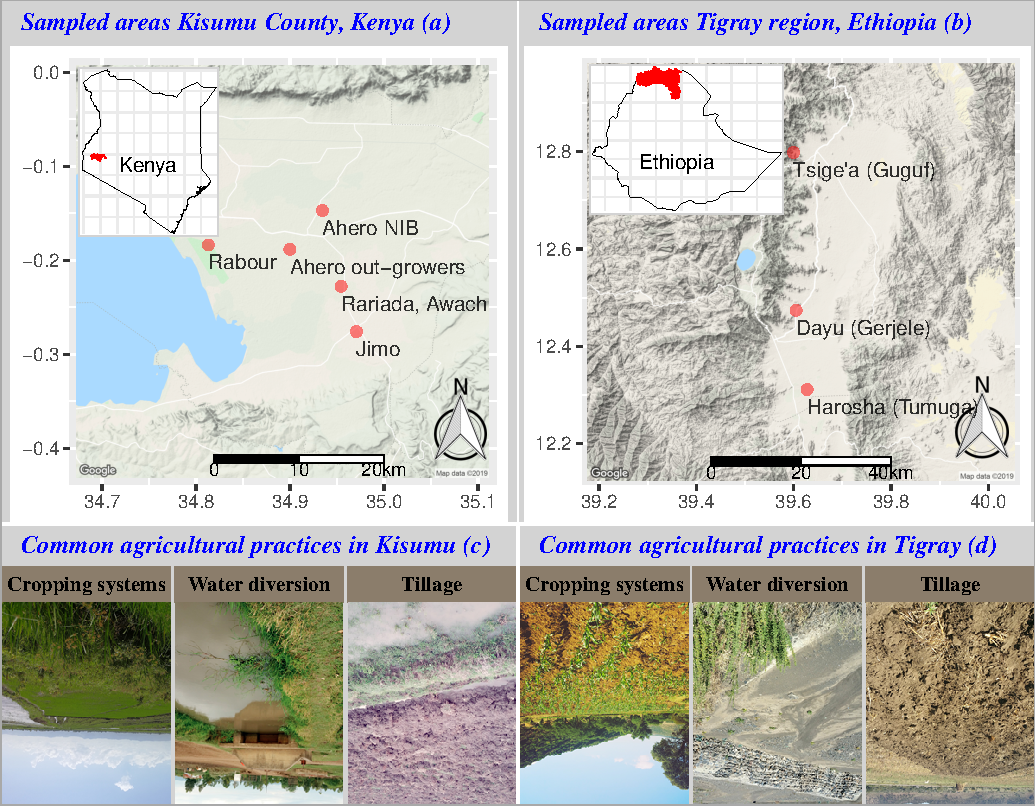
\includegraphics[width=1\linewidth,]{figures/Modelling_FBFS_study_area} 

}

\caption{Description of the sampling frame used to develop a mixed model of various flood-based farming practices in the Tigray region of Ethiopia and Kisumu County in Kenya. Agricultural practices are mainly homogeneous within study regions. The term 'out-growers' refers to farmers outside the scope of the Kenyan national irrigation board. Traditional flood water diversions are physical infrastructure, such as deflecting spurs or soil bunds that are constructed by farmers across flood channels using locally available materials. Modern diversion structures, such as diversion weirs, are usually designed by engineers and made of concrete. The improved diversion type constitutes an integration of farmer and engineer knowledge.}\label{fig:fig1}
\end{figure}

\begin{itemize}
\item
  Ahero and Awach out-growers (Kisumu): here water is acquired via simple gravity from the Nyando and Awach Rivers. The main difference between these locations is that the Ahero out-growers scheme serves as safe disposal for excess water in East Kano.
\item
  East Nyankach (Kisumu): in this location, water is collected via runoff and roof water harvesting. Typically, the collected water is stored in various household ponds and water tanks to later be used for irrigation.
\item
  Tsige'a, Harosha, and Dayu (Tigray): in these locations, farmers use improved, traditional, and modern floodwater diversions, respectively, to harness spate flow from various dry wadis.
\end{itemize}

The differences captured in these eight areas (Figure \ref{fig:fig1} c, d, e) have implications for water supply, social organization, and crop development. For example, risks related to water supply may be more prominent in the out-growers' schemes, which are exposed to water excess and shortages, compared to the schemes managed by the Kenyan national irrigation board, where the water supply is more regulated. While the water sources and acquisition procedures vary among rice-based systems in Kisumu (i.e.~out-growers, East and West Kano), cultural practices are similar. In these areas, rice is sown (after tillage and flooding) in monoculture during floods, followed by various types of flood recession crops that are intercropped depending on farmers' preferences and water availability (Figure \ref{fig:fig1} c). In Tigray, in contrast, crops (mainly maize, sorghum and teff) are sown based on rainfall and are later irrigated using flood water (Figure \ref{fig:fig1} d).

\hypertarget{ref3}{%
\section{Methods}\label{ref3}}

\hypertarget{ref31}{%
\subsection{Participatory model development}\label{ref31}}

To describe crop performance within FBFS settings, we developed a mixed Bayesian Network / Monte Carlo model describing causal relationships deemed important for crop production in FBFS. We parameterized the model using various sources of information, including literature, online databases, expert knowledge elicitation, farmer and expert interviews and remote sensing (Krueger et al., 2012; Refsgaard et al., 2007). To ensure quality in their estimations, experts were introduced to the principles of decision analysis and subjected to calibration training (Hubbard, 2014; Luedeling et al., 2015; Whitney, Lanzanova, et al., 2018; Whitney, K. Shepherd, et al., 2018).

\begin{figure}[!h]

{\centering 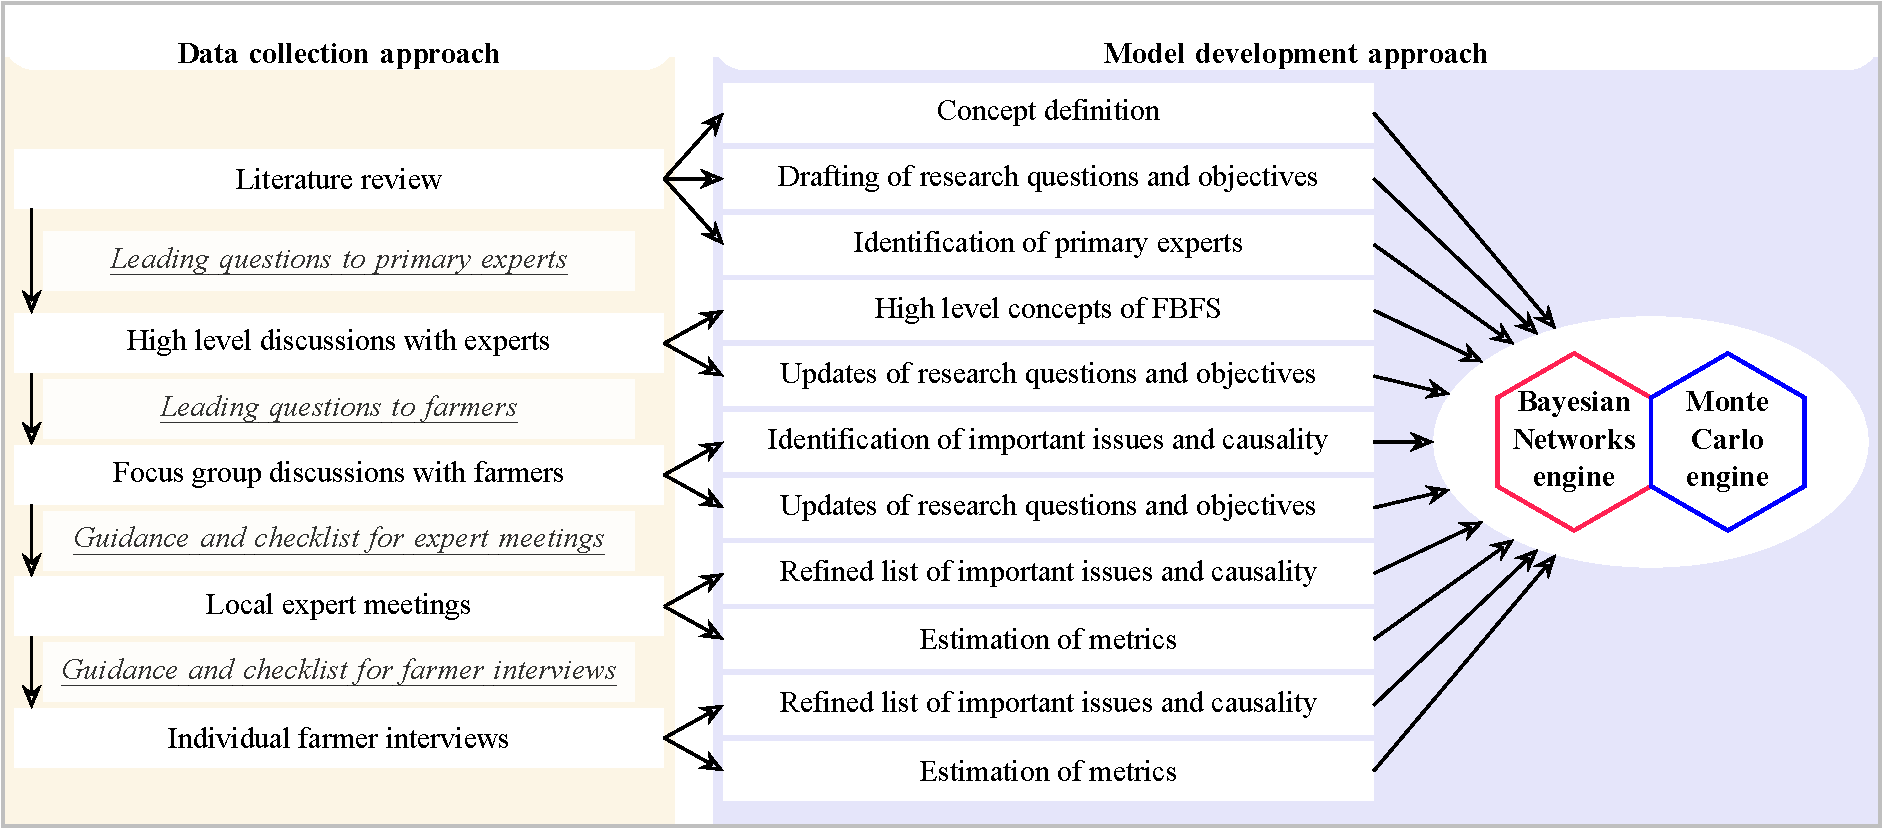
\includegraphics[width=1\linewidth,]{figures/fig2-plot-1} 

}

\caption{Overview of the approach used to develop a crop model for flood-based farming systems in the Tigray region of Ethiopia and Kisumu County in Kenya.}\label{fig:fig2}
\end{figure}

The model development process consisted of five sequential steps with specific milestones (Figure \ref{fig:fig2}) aiming to develop theories that match farmers' realities:

\begin{enumerate}
\def\labelenumi{\arabic{enumi}.}
\item
  Literature review to understand the issue and design broad leading questions to primary experts (experts from various academic and research institutions working with FBFS and related fields).
\item
  High-level discussions with 11 primary experts aiming to develop a general understanding of important FBFS concepts.
\item
  Discussions with 20 focus groups in Ahero and Kisumu towns (Kenya) in December 2016 and June 2017 and in Mekelle and Alamata towns (Ethiopia) in December 2016 and January 2017.
\item
  Consultation with local experts to formalize the model. The pool of local experts, initially represented by local farmers and extension civil servants, was extended to include the participants of a leadership course in flood-based farming and water harvesting in Kenya and the participants of the International Training Course on Integrated Watershed Management and FBFS in Ethiopia (FBLN, 2018).
\item
  Interviews with 159 farmers to capture farmers' realities in the model.
\end{enumerate}

The experts were selected based on their relevant and extensive experience regarding the practice of FBFS (Krueger et al., 2012). The information acquired in the first four steps was made available to the local experts to formalize the model. Qualitative variables were interlinked using BNs, whereas the quantitative ones were connected using MC models (Figure \ref{fig:fig2}; Figure \ref{fig:fig3}). The BNs and MC models were connected to form generic models that account for the variability of the FBFS schemes in each study region. These models were further merged into a single generic model that captures the variability in the study regions. Our goal was to develop a detailed description of the system by breaking down the system complexity into all important processes (see section \ref{ref34}) while highlighting risk factors that influence crop production and fully accounting for data uncertainty (Refsgaard et al., 2007; Van Den Ham, 2008).

\hypertarget{ref32}{%
\subsection{Models for quantitative variables}\label{ref32}}

An MC simulation is a quantitative procedure used to estimate the values of continuous variables. Its centrepiece is a deterministic mathematical equation that contains one or more input variables, whose values are expressed as probability distributions. Outputs are generated by drawing many sets of random values from these distributions and using these to parameterize the central equation. The population of outputs across the whole set of calculations expresses a reasonable estimate of uncertainty around the value of the target output variable (Luedeling et al., 2015; Refsgaard et al., 2007; Rosenstock et al., 2014).

MC models were used to describe quantitative biomass accumulation during crop development and the conversion of this biomass into grain. The MC expert system is based on the concept of yield potential, which is the theoretical yield limit of a variety grown under optimal conditions (Van Ittersum et al., 2013). Since achieving the full yield potential is unrealistic, the MC models considered the exploitable yield potential as the fraction of yield potential (70 -- 80\%) that could potentially be achieved by farmers under ideal conditions. Since such ideal conditions are not encountered in most places, the models considered the attainable yield potential to account for the systemic constraints encountered on farms. Finally, the expected actual yield was determined as the yield expectation given a farmer's management conditions (Van Ittersum et al., 2013). The models involving deterministic relationships between these yield metrics were used for MC simulations.

\hypertarget{ref33}{%
\subsection{Models for qualitative variables}\label{ref33}}

BNs are multivariate cause-effect models suitable for conditional reasoning across variables with multiple qualitative states. They can be used to specify the probabilities of the states of unknown discrete variables, conditional on the probabilities of the states of other variables. These conditional probabilities express causal relationships between the discrete variables (Jensen, 1996; Pearl, 1988). BNs are composed of logical connections (directed edges) between variables (nodes), which are arranged in probabilistic graphical models. Dependencies are represented by arrows (arcs) encoding the direction and nature (i.e.~direct or indirect) of the causal relationships (Pearl, 1988). A node describes the states of a variable (node states), with a variable at the arrowhead (child node) being influenced by the variable at the arrow tail (parent node). The strength of the influence is portrayed by the conditional probabilities typically specified as stochastic matrices known as conditional probability tables (CPTs), which are the central elements of BNs (Fenton and Neil, 2013; Jensen, 1996; Pearl, 1988). They portray the strength of the association between all states of a child node and the various states of its parents (Hansson and Sjökvist, 2003; Scutari and Denis, 2015).

The BNs developed by the local experts detailed complex causalities defining one important variable: the `farming constraints' factor, which accounts for the combined effects of all limiting factors. The BN expert systems are based on the idea that system functions are driven by various biotic and abiotic factors that depend on management practices (Jax and Setälä, 2005). These profile a given farmland in terms of farming constraints and performance. The effects of farming constraints were defined at plot level with implications for farming systems. The `farming constraints' variable was produced with the help of BNs to summarize qualitative expert knowledge for use in quantitative MC simulations.

\hypertarget{ref34}{%
\subsection{Modularity and system complexity}\label{ref34}}

The generic model encapsulates the complexity of the farming system in four levels of abstractions embedded in the BN and MC models:

\begin{enumerate}
\def\labelenumi{\arabic{enumi}.}
\item
  Recognition of individual processes defining system performance: This was done in plenary sessions during workshops, where the important processes were identified and formulated as separate modules based on the assumption that farming constraints affect crop development on any given plot. The farming constraints variable was estimated via the BNs using three modules: the soil water, the cropping system and the management modules. These processes were described through causal chains describing resource allocation (e.g.~available soil water or available soil nutrients) within the system. Crop development, in turn, was assessed via the MC model using a single module, the crop growth module. In most cases, these complex processes were described in terms of their corresponding sub-processes (as sub-modules) to facilitate the description of the main process.
\item
  Disaggregation of the processes into individual variables (e.g.~rainfall occurrence or manure application): This was done in working groups with the aim of identifying important variables and interfaces for shared connections between the processes.
\item
  Description of the variables: This was also done in working groups with the aim of defining the relationships between variables and estimating their values. Quantitative variables were estimated as continuous probability distributions. Qualitative variables were disaggregated into their respective states (e.g.~it rains or it does not, manure is either applied or it is not), for which state probabilities were estimated as CPTs (see section \ref{ref35}). The variability among system processes across farmlands is considered to imply differences in the states of variables modulating them. The full BN and MC models describing these are provided in the technical and supplementary materials.
\item
  Separation of crop development into critical stages: Crop development stages were defined from the onset of the cropping season to 10\% ground cover as initial stage, from 10\% ground cover to effective full cover as the development stage, from effective full cover to the start of maturity as the mid stage, and from the start of maturity to harvest or full senescence as the late stage (Allen et al., 1998). A biomass expansion factor, measuring crop growth, was considered to control the crop growth at each of these stages. This way, crops would not arbitrarily grow beyond the actual yield expectations. Crop yield was assumed to follow a negatively skewed gamma distribution (Gallagher, 1987; Ramirez et al., 2003), meaning that there is a high chance of low yield and relatively low chance of high yield. Four crops -- rice, maize, sorghum and teff -- were considered due to their importance in the study areas.
\end{enumerate}

\hypertarget{ref35}{%
\subsection{Modelling interface}\label{ref35}}

The make\_CPT function from the decisionSupport package in R was used to facilitate the estimation of the CPTs (Luedeling et al., 2019). To create the full CPT, the function requires the prior probability distribution of the child node, the child node's sensitivity relative to the parents, the parents' effects, and the weight of influence of each parent (Luedeling et al., 2019). These parameters were estimated by the experts (Hansson and Sjökvist, 2003; Whitney, K. Shepherd, et al., 2018). The make\_CPT routines were automated and interfaced with the cptable function from the gRain package (Højsgaard, 2012) to formalise the BNs in computer-readable graphical models following the experts' causal reasoning.

While BNs are ideal for specifying complex levels of hierarchy and categorization as cause-effect relationships, they provide a convenient interface for studying simple aspects based on the states of different variables and their causal linkages. Based on the different combinations of the states of its parents, the probabilities of the `farming constraint' node were generated by sampling from the posterior distributions of the BNs. This is equivalent to generating all possible farming constraint scenarios based on the BN models. Technically, we used MC particle filters (Kitagawa, 1996; Koller and Friedman, 2009; Scutari, 2010) to generate the probabilities of farming constraints conditional on different combinations of the states of variables involved in the BNs. The effects of the different states of the variable were assumed to range between 0 and 1, where 0 denotes ideal conditions (exploitable yield potential) and 1 the worst-case scenario (total loss). The variable was used as special node in the MC model as expected loss ratio, accounting for both the effects of the variable states and their probability of occurrence (Figure \ref{fig:fig3}).

\begin{figure}[!h]

{\centering 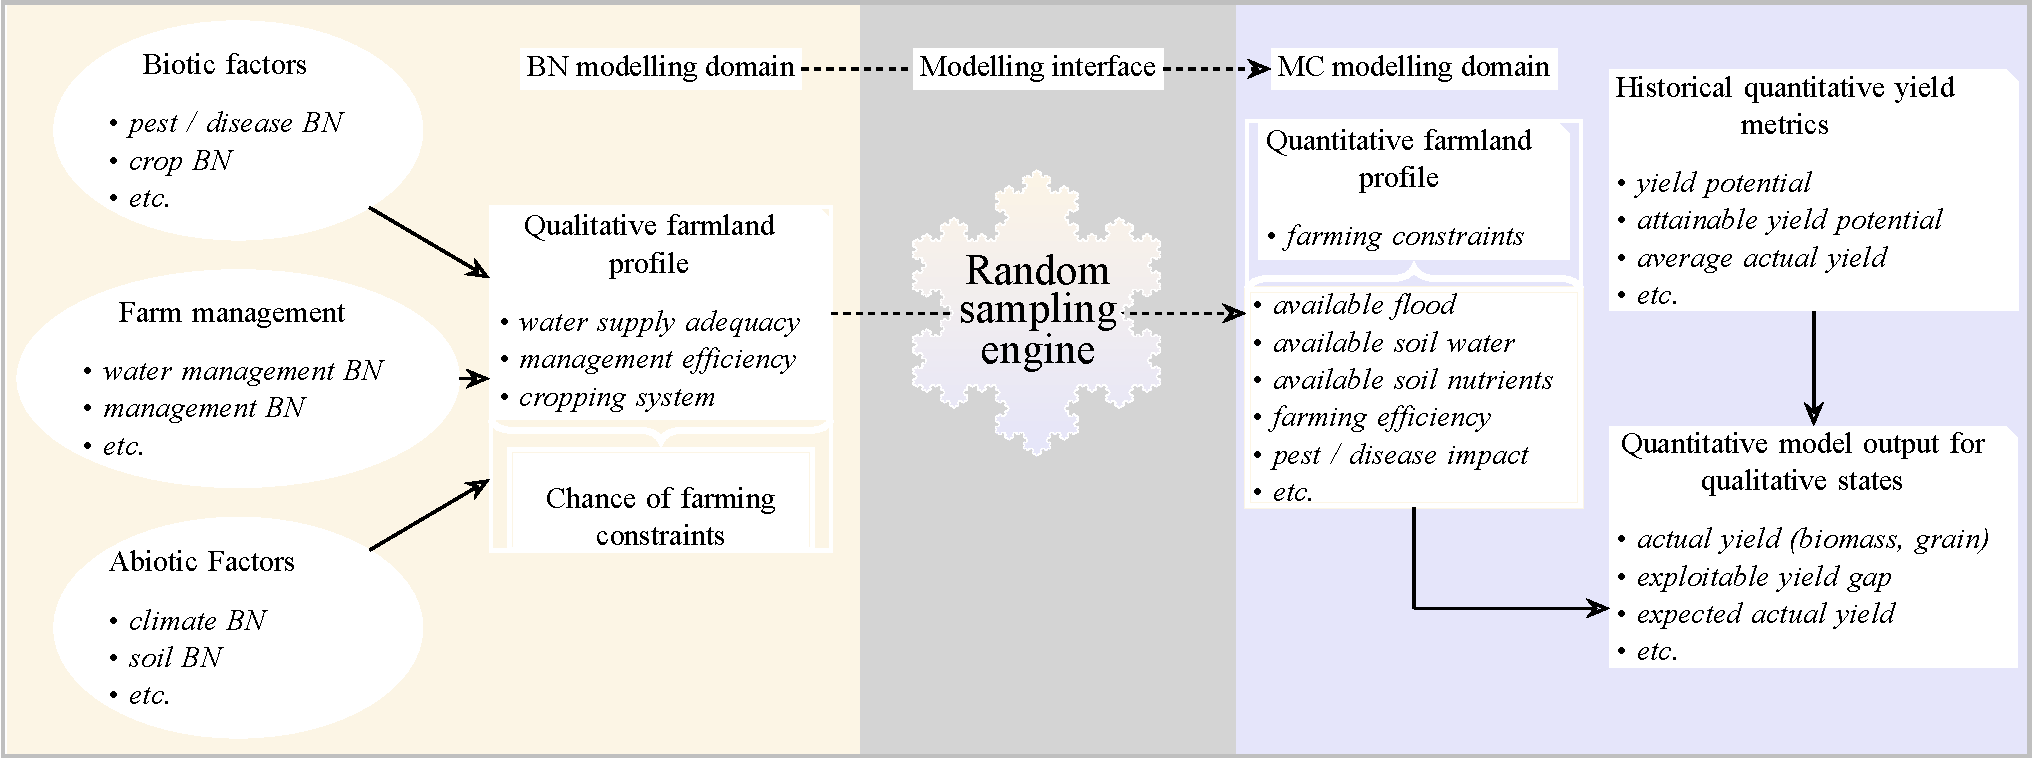
\includegraphics[width=1\linewidth,]{figures/fig3-plot-1} 

}

\caption{Conceptual framework of important processes considered in the development of a crop model for flood-based farming systems in the Tigray region of Ethiopia and Kisumu County in Kenya.}\label{fig:fig3}
\end{figure}

A combination of MC and BN models is ideal for specifying complex deterministic and cause-effect relationships while enabling the use of data and information that are not necessarily precise. These modelling approaches can produce reliable advice that makes full use of the current state of information and adequately expresses all uncertainties in such a way that outcomes and risks of a given decision can be appreciated. While the MC expert system was set to simulate the various yield metrics (Figure \ref{fig:fig3}) ranging from the maximum possible yield to what farmers actually achieve (Van Ittersum et al., 2013), the BNs were programmed to provide the shape of the probability distributions of the variable `farming constraint' (Figure \ref{fig:fig3}), as well as its 90\% confidence interval and median values. This was done at each of the four crop development stages to account for the variability of farming constraints over the growing season and the biomass accumulation over time.

Note that the probability distributions of the node `farming constraints' were determined based on reasonable bounds for skewness and kurtosis defined via visual observations supported by bootstrapping (Delignette-Muller and Dutang, 2015). We fitted several candidate distributions using the fitdist function from the fitdistrplus package (Delignette-Muller and Dutang, 2015), from which we chose the best-fitting distribution. In the supplementary materials, we show examples of Cullen and Frey graphs, quantile and probability plots along with the theoretical and empirical density and cumulative distribution functions used to facilitate the choice of the distributions. Note also that the remaining parameters required by decisionSupport's mcSimulation function (Luedeling et al., 2019), which was used to conduct the MC simulation, were computed from the fitted distribution using the fitdist function and other facilities provided by the rriskDistributions package (Belgorodski et al., 2017).

\hypertarget{ref36}{%
\subsection{Inputs, outputs and special models}\label{ref36}}

The generic model was used to demonstrate the flexibility of the approach and the importance of modularity in customizing model behaviour for specific situations. The results of the specific models were used to present the different modules and their throughputs using three case studies of varying complexity:

\begin{enumerate}
\def\labelenumi{\arabic{enumi}.}
\item
  The assessment of soil water using the soil water module looks at the challenge of maximizing water storage in soils, while limiting waterlogging and restricting water losses through evaporation, run-off or percolation in FBFS. We show how the model can be customized to prescribe optimum pre-season cultural practices for improved soil water on specific soil types.
\item
  The probabilistic assessment of crop biomass uses the crop growth module to show the model's suitability as monitoring tool for biomass accumulation over the growing season.
\item
  The study of the impact of soil water and biotic stresses (e.g.~pest, diseases and weeds) shows the effects of these on the grain yield of rice and sorghum, integrating use of all four model modules.
\end{enumerate}

Inputs consisted of scenarios that were formulated based on child-parent state relationships. Outputs are the probability of adequate soil water, biomass and grain yield, respectively. The rationale and methodology of each of these case studies are provided in the supplementary materials.

\hypertarget{ref4}{%
\section{Results}\label{ref4}}

\hypertarget{ref41}{%
\subsection{Overview of the Conceptual Model}\label{ref41}}

The generic model (overview in Figure \ref{fig:fig4}) interlinking the four modules that describe the important processes at plot level is composed of 121 nodes in the BNs and 21 nodes in the MC model. The full model is provided as reproducible code in the technical materials. Customized instances showing the usefulness and usability of the approach are presented in the following sections to demonstrate the functioning of the model. The four modules represent individual processes describing the soil water, the cropping system, farm management, and the crop growth, which are linked by various connectors (Figure \ref{fig:fig4}).

\begin{figure}[!h]

{\centering 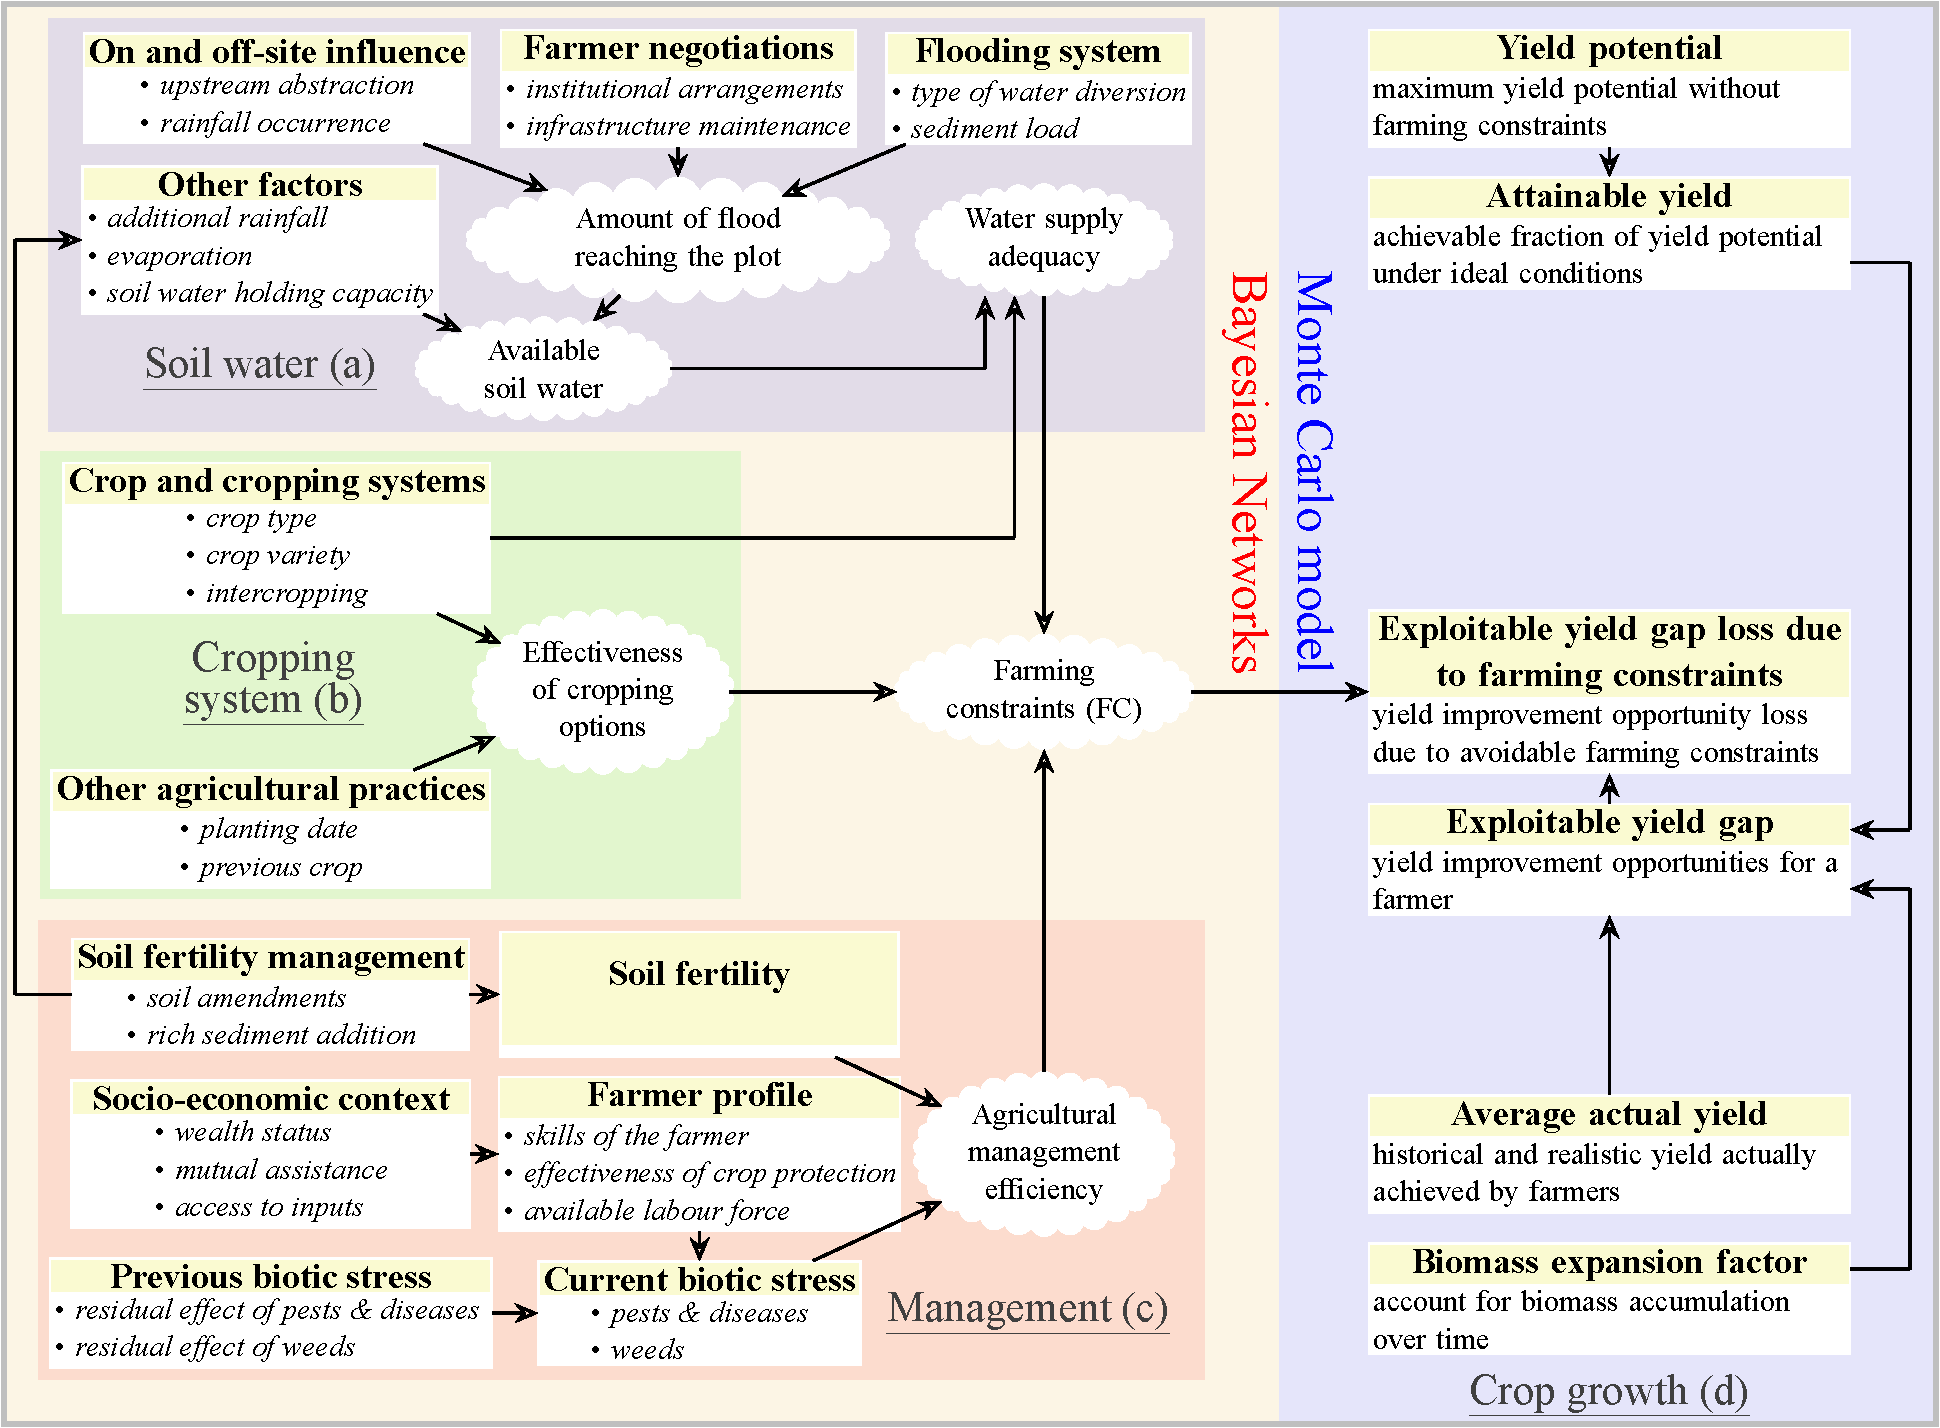
\includegraphics[width=1\linewidth,]{figures/fig4-plot-1} 

}

\caption{Overview of the mixed Bayesian Network/Monte Carlo crop model for flood-based farming systems in the Tigray region of Ethiopia and Kisumu County in Kenya. a) factors determining the available soil water, b) cropping system characteristics, c) management practices adopted by the farmer, and d) crop development over time. This graph provides a simplified overview of the generic model. Nodes represent groupings of similar aspects. Bullet lists only provides example of variables that can be expected in the model described in fine detail in the technical material. Bubble shapes are Bayesian networks formed by variables (rectangular shapes) pointing to them.}\label{fig:fig4}
\end{figure}

\hypertarget{ref42}{%
\subsection{Soil water module}\label{ref42}}

The soil water module (Figure \ref{fig:fig4} a) aims to estimate the adequacy of water supply to the crop, which was judged a convenient determinant of crop performance (in the sense of water-limited yield). Adequacy is related to available soil water, which is positively influenced by other factors such as rainfall, soil water holding capacity and the amount of flood reaching the plot, and negatively affected by evaporation (Figure \ref{fig:fig5}). Two sub-modules were used to describe this module: the amount of flood reaching the plot, and the available soil water (see supplementary material). The former describes external influences, infrastructure, and social arrangements determining flood water acquisition and sharing in FBFS. The latter describes the factor `soil water', as it would be described under rainfed conditions (Figure \ref{fig:fig5}).

The amount of flood obtained by a farmer depends on agreements for water sharing and system maintenance between stakeholders. These can reduce sediment loads (depending on the type of water diversion), with positive implications for the adequacy of water supply to crops. External effects such as upstream abstraction can reduce the amount of flood reaching the plot directly or indirectly (via the amount of shared flood water). Off-site rainfall occurrence can have a positive effect by increasing water supply. Soil water availability, however, is not only defined by these aspects; it also relies on intrinsic soil characteristics, farmer management, and other climatic factors (Figure \ref{fig:fig5}).

\begin{figure}[!h]

{\centering 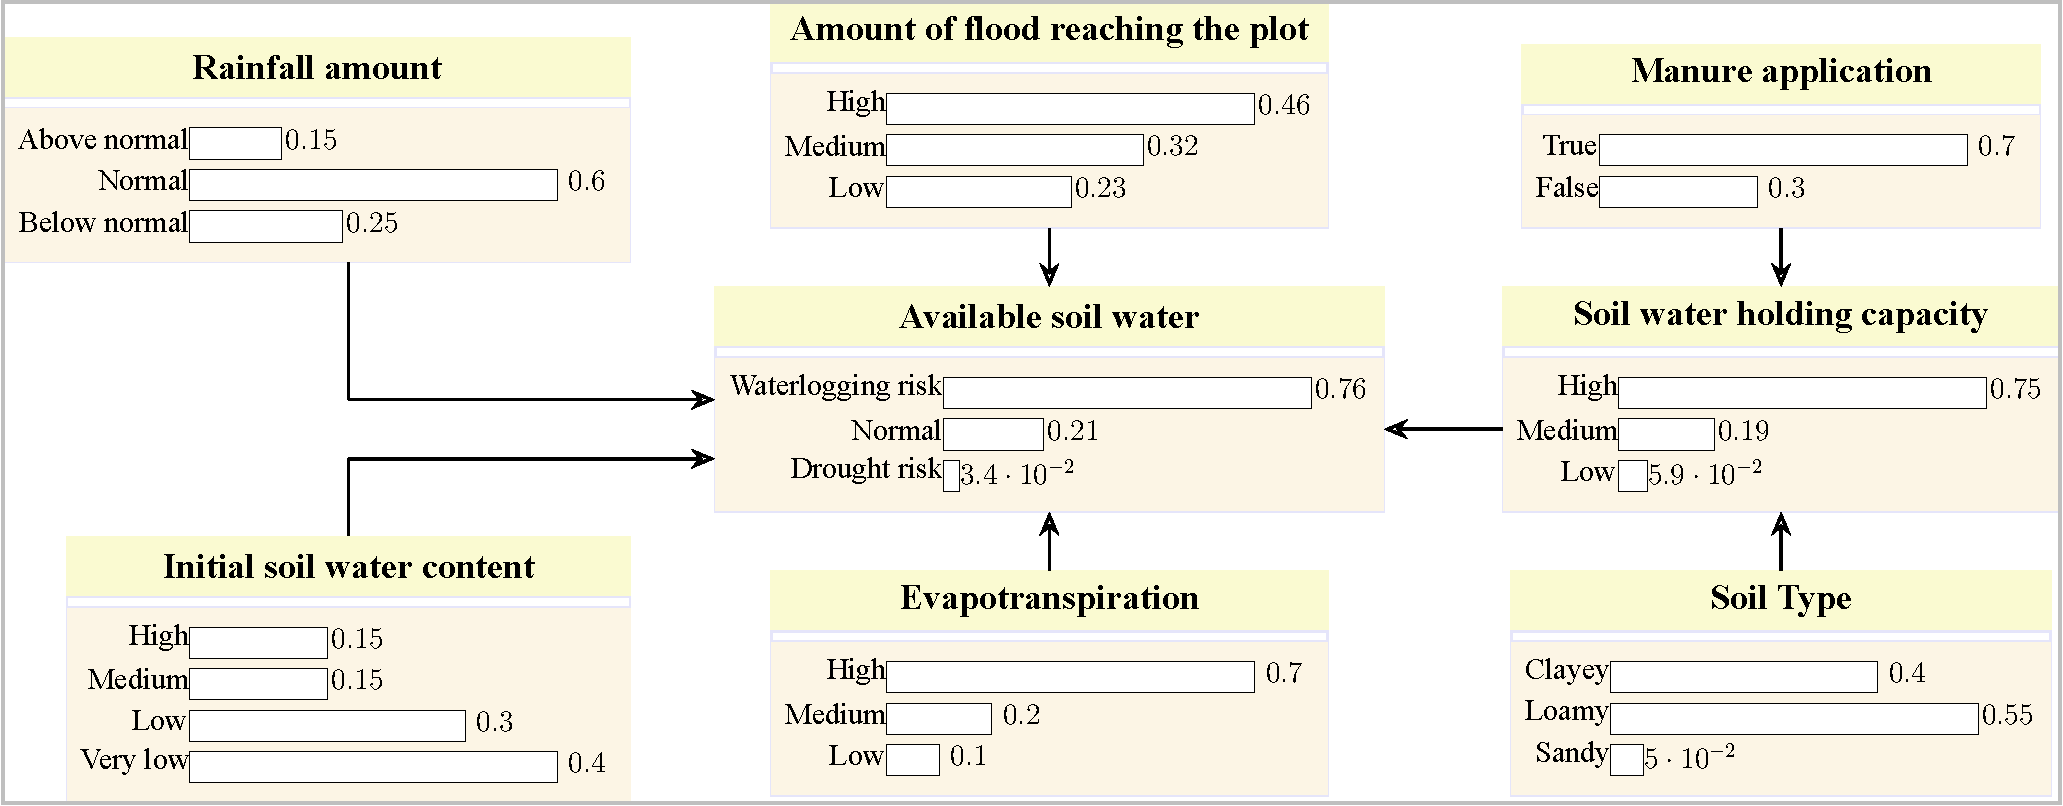
\includegraphics[width=1\linewidth,]{Modelling_FBFS_files/figure-latex/fig5-plot-1} 

}

\caption{Causal linkages defining the factor ‘available soil water content’ in flood-based farming systems in the Tigray region of Ethiopia and Kisumu County in Kenya (simplified illustration).}\label{fig:fig5}
\end{figure}

The assessment of soil water using the soil water module (Figure \ref{fig:fig6}) shows that on clayey soils without manure application, drought is unlikely to occur, while waterlogging is very likely when at least the desired amount of floodwater is obtained (Figure \ref{fig:fig6}). Uncertainty is greater when little floodwater is available. Supplementary manure application slightly increases the chance of waterlogging, which also increases when too much floodwater is obtained.

Loamy soils generally behave similarly to clayey ones, with a slightly lower chance of waterlogging and greater probability of normal soil water conditions. Sandy soils (the dominant soil type in FBFS) appear to be the riskiest and most uncertain soil type for soil water. Drought is likely in years with little floodwater and manure application.

\begin{figure}[!h]

{\centering 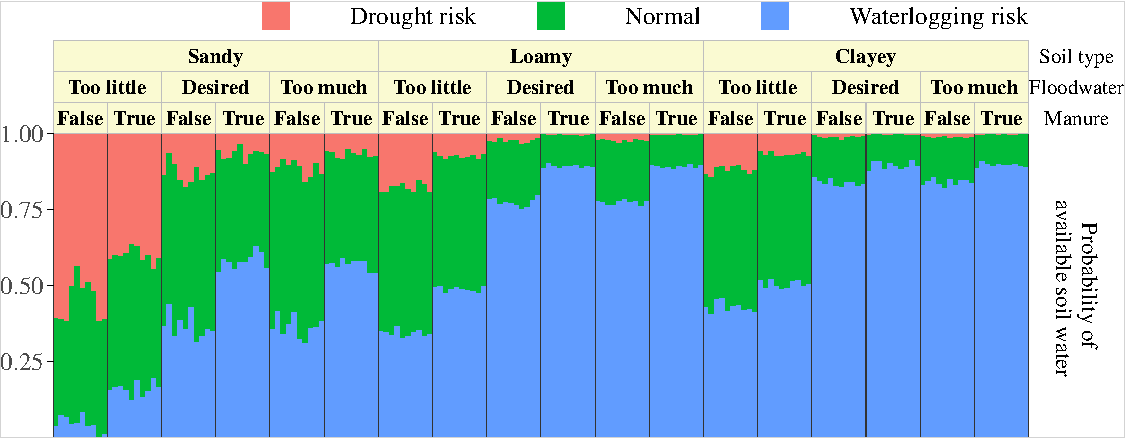
\includegraphics[width=1\linewidth,]{figures/Modelling_FBFS_factor_of_soil_water} 

}

\caption{Effect of soil type, manure, and flood water on available soil water in flood-based farming systems in the Tigray region of Ethiopia and Kisumu County in Kenya. Each block represents 10 possible outcomes of the corresponding query. Each query was run 1000 times.}\label{fig:fig6}
\end{figure}

\hypertarget{ref43}{%
\subsection{Cropping system module}\label{ref43}}

The cropping system module (Figure \ref{fig:fig4} b) aims to assess the effectiveness of the cropping options, evaluating the performance of the cropping system adopted by the farmer instead of the cropping system itself. Crop types were ranked in decreasing order of yield (rice, teff, maize and sorghum) with improved crop varieties assumed to perform better than local ones. However, the effectiveness of the cropping system depends on an array of agricultural practices such as the choice of planting date, the crops previously grown on the same land, and the presence and density of intercropping. The most effective cropping is generally achieved when an improved variety is planted early on land that had a different crop in the previous season. This can depend on the crop type. For example, rice and teff are quite tolerant of repeated cultivation and monoculture, whereas maize and sorghum perform better in crop rotations and intercropping.

\hypertarget{ref44}{%
\subsection{Crop growth module}\label{ref44}}

The crop growth module (Figure \ref{fig:fig4} d; Figure \ref{fig:fig7}) monitors biomass accumulation over time to provide estimates of yield metrics (e.g.~biomass yield gap, exploited biomass yield) at different stages of crop development. Figure \ref{fig:fig7} summarises the MC model including the relationships between the quantitative variables and the mathematical calculations involved at the initial and development stages. Crops are initially regarded in terms of their boundary conditions represented by their yield potential, which was differentiated into attainable yield potential, yield gaps, and actual yield via the actual farm conditions represented by farming constraints (see section \ref{ref32}; Figure \ref{fig:fig7}). The simulation produced 324 outcomes corresponding to the different scenarios described in section \ref{ref36}. Only a few of these results are presented here to showcase the model. We selected the initial and the late stages of crop development along with the worst, medium, and best-case scenarios to show the biomass accumulation over time, and to illustrate the effect of varying farming constraints on crop development (Figure \ref{fig:fig8}).

\begin{figure}[!h]

{\centering 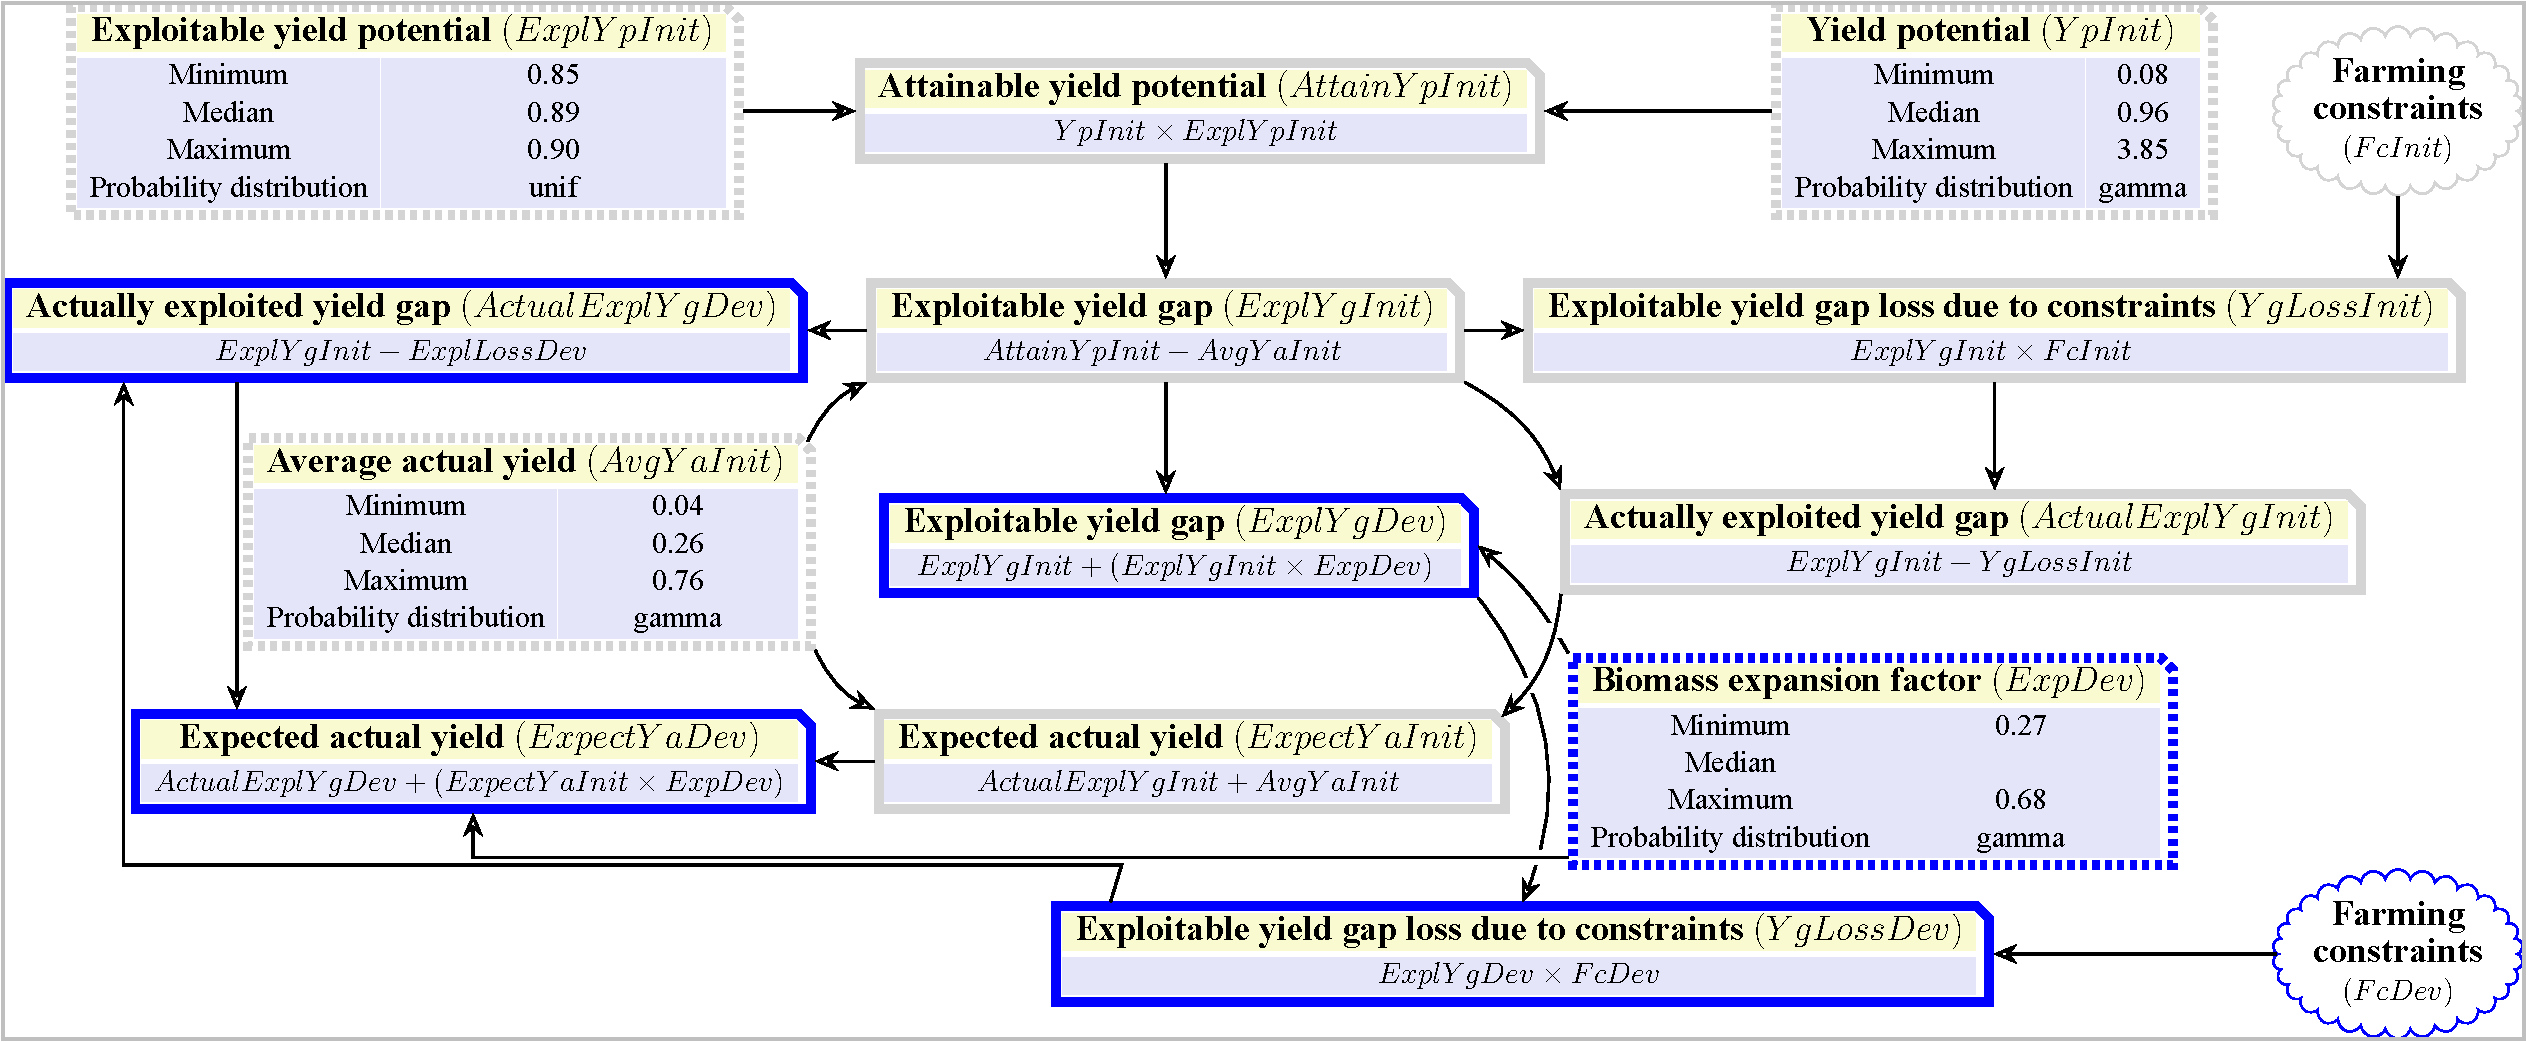
\includegraphics[width=1\linewidth,]{Modelling_FBFS_files/figure-latex/fig7-plot-1} 

}

\caption{Overview of a Monte Carlo model assessing biomass accumulation during crop development in flood-based farming systems in the Tigray region of Ethiopia and Kisumu County in Kenya. Gray-bordered nodes are taken at initial stage. Blue-bordered nodes are taken at development stage. Dashed and plain lines nodes, respectively, are elicited and computed.}\label{fig:fig7}
\end{figure}

The probabilistic assessment of crop biomass shows that simulated actual biomass yield, as well as the other yield metrics, were affected by several risk factors (Figure \ref{fig:fig8}), some of which are specific to FBFS. Farms generally have a high probability of relatively low yield, which varies substantially over time and in response to differing levels of farming constraints.

Based on computed 90\% confidence intervals, the exploitable yield gap, the actually exploited yield gap, and the expected yield can differ by a factor of two between situations with high and low farming constraints. The exploitable yield gap and loss due to farming constraints are substantial, indicating great potential for yield improvement. Exploitable yield loss is positively correlated with farming constraints, with a high chance of zero loss under minimal farming constraints. Simulation results show right-skewed gamma distributions (Figure \ref{fig:fig8}) indicating that crop yields in the study area are characterized by a relatively high frequency of low values. This highlights important uncertainty regarding yield expectations in the study areas. In general, chances of grain yield above 5 t/ha are negligible.



\begin{figure}[!h]

{\centering 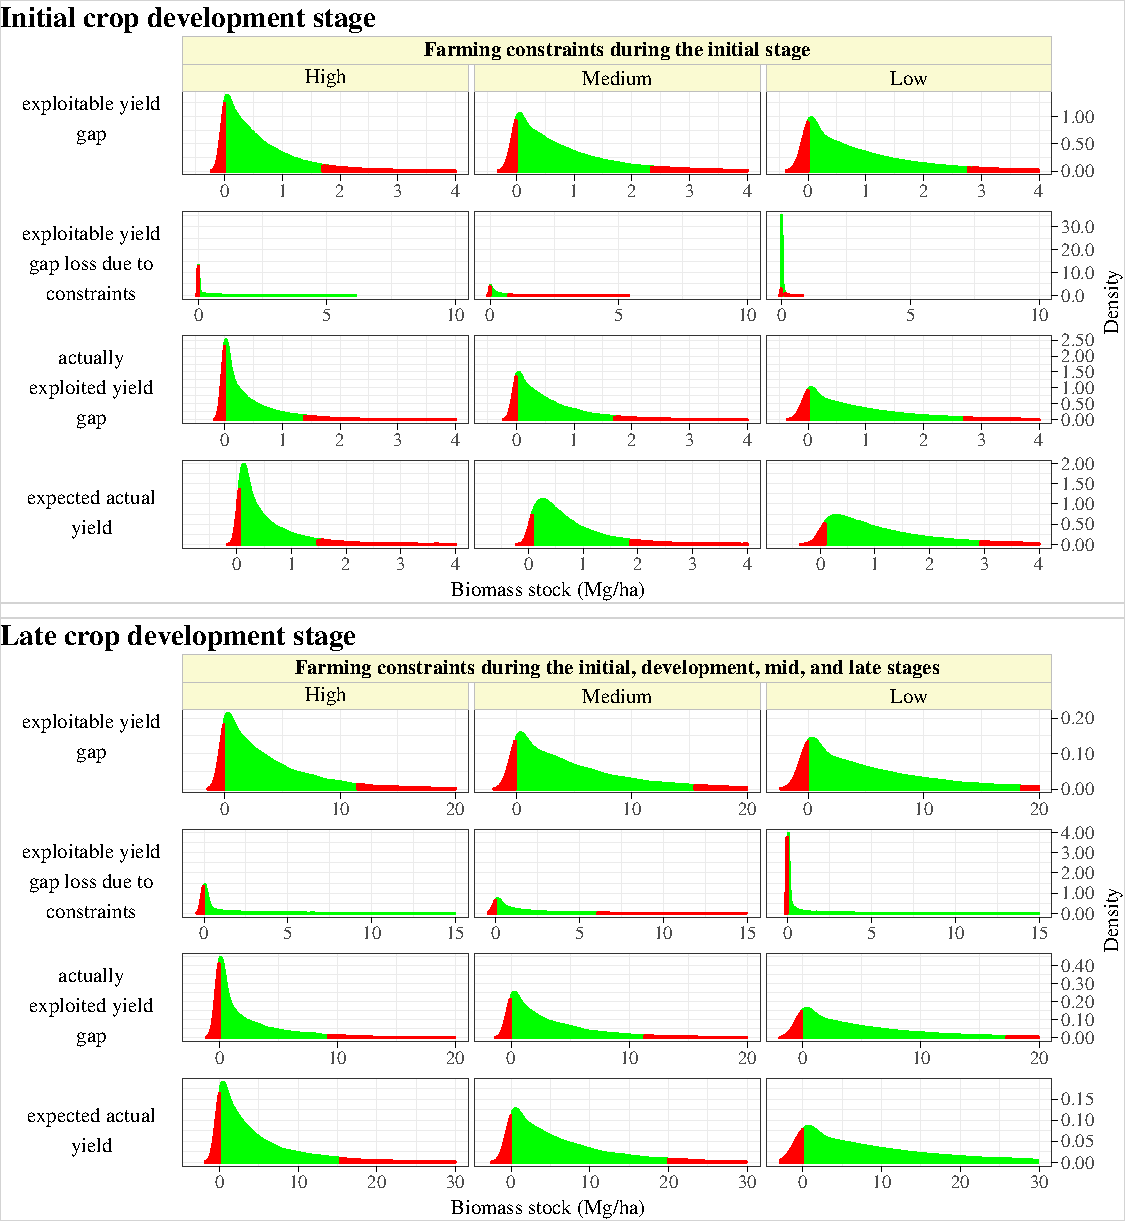
\includegraphics[width=1\linewidth,]{figures/Modelling_FBFS_biomass_yield_Initial_and_late_stage} 

}

\caption{Simulated biomass yield metrics for flood-based farming systems in the Tigray region of Ethiopia and Kisumu County in Kenya. The green and red colors, respectively, are values inside and outside the 90\% confidence interval.}\label{fig:fig8}
\end{figure}

\hypertarget{ref45}{%
\subsection{Management module}\label{ref45}}

The management module (Figure \ref{fig:fig4} c) points out the agricultural management efficiency via four important sub-modules describing the general household situation, soil nutrients, pests \& diseases, and weeds (Figure \ref{fig:fig4} c; Figure \ref{fig:fig9}). Pest \& disease attacks can weaken the crop in subsequent development stages, aggravating other problems and ultimately lowering the agricultural management efficiency, particularly when the farmer lacks advanced skills in crop protection. The skill of the farmer, which is determined by the social and economic context (e.g.~opportunity, willingness, and ability to purchase inputs), defines the management efficiency in terms of water and crop protection methods adopted by the farmer (Figure \ref{fig:fig4} c).

\begin{figure}[!h]

{\centering 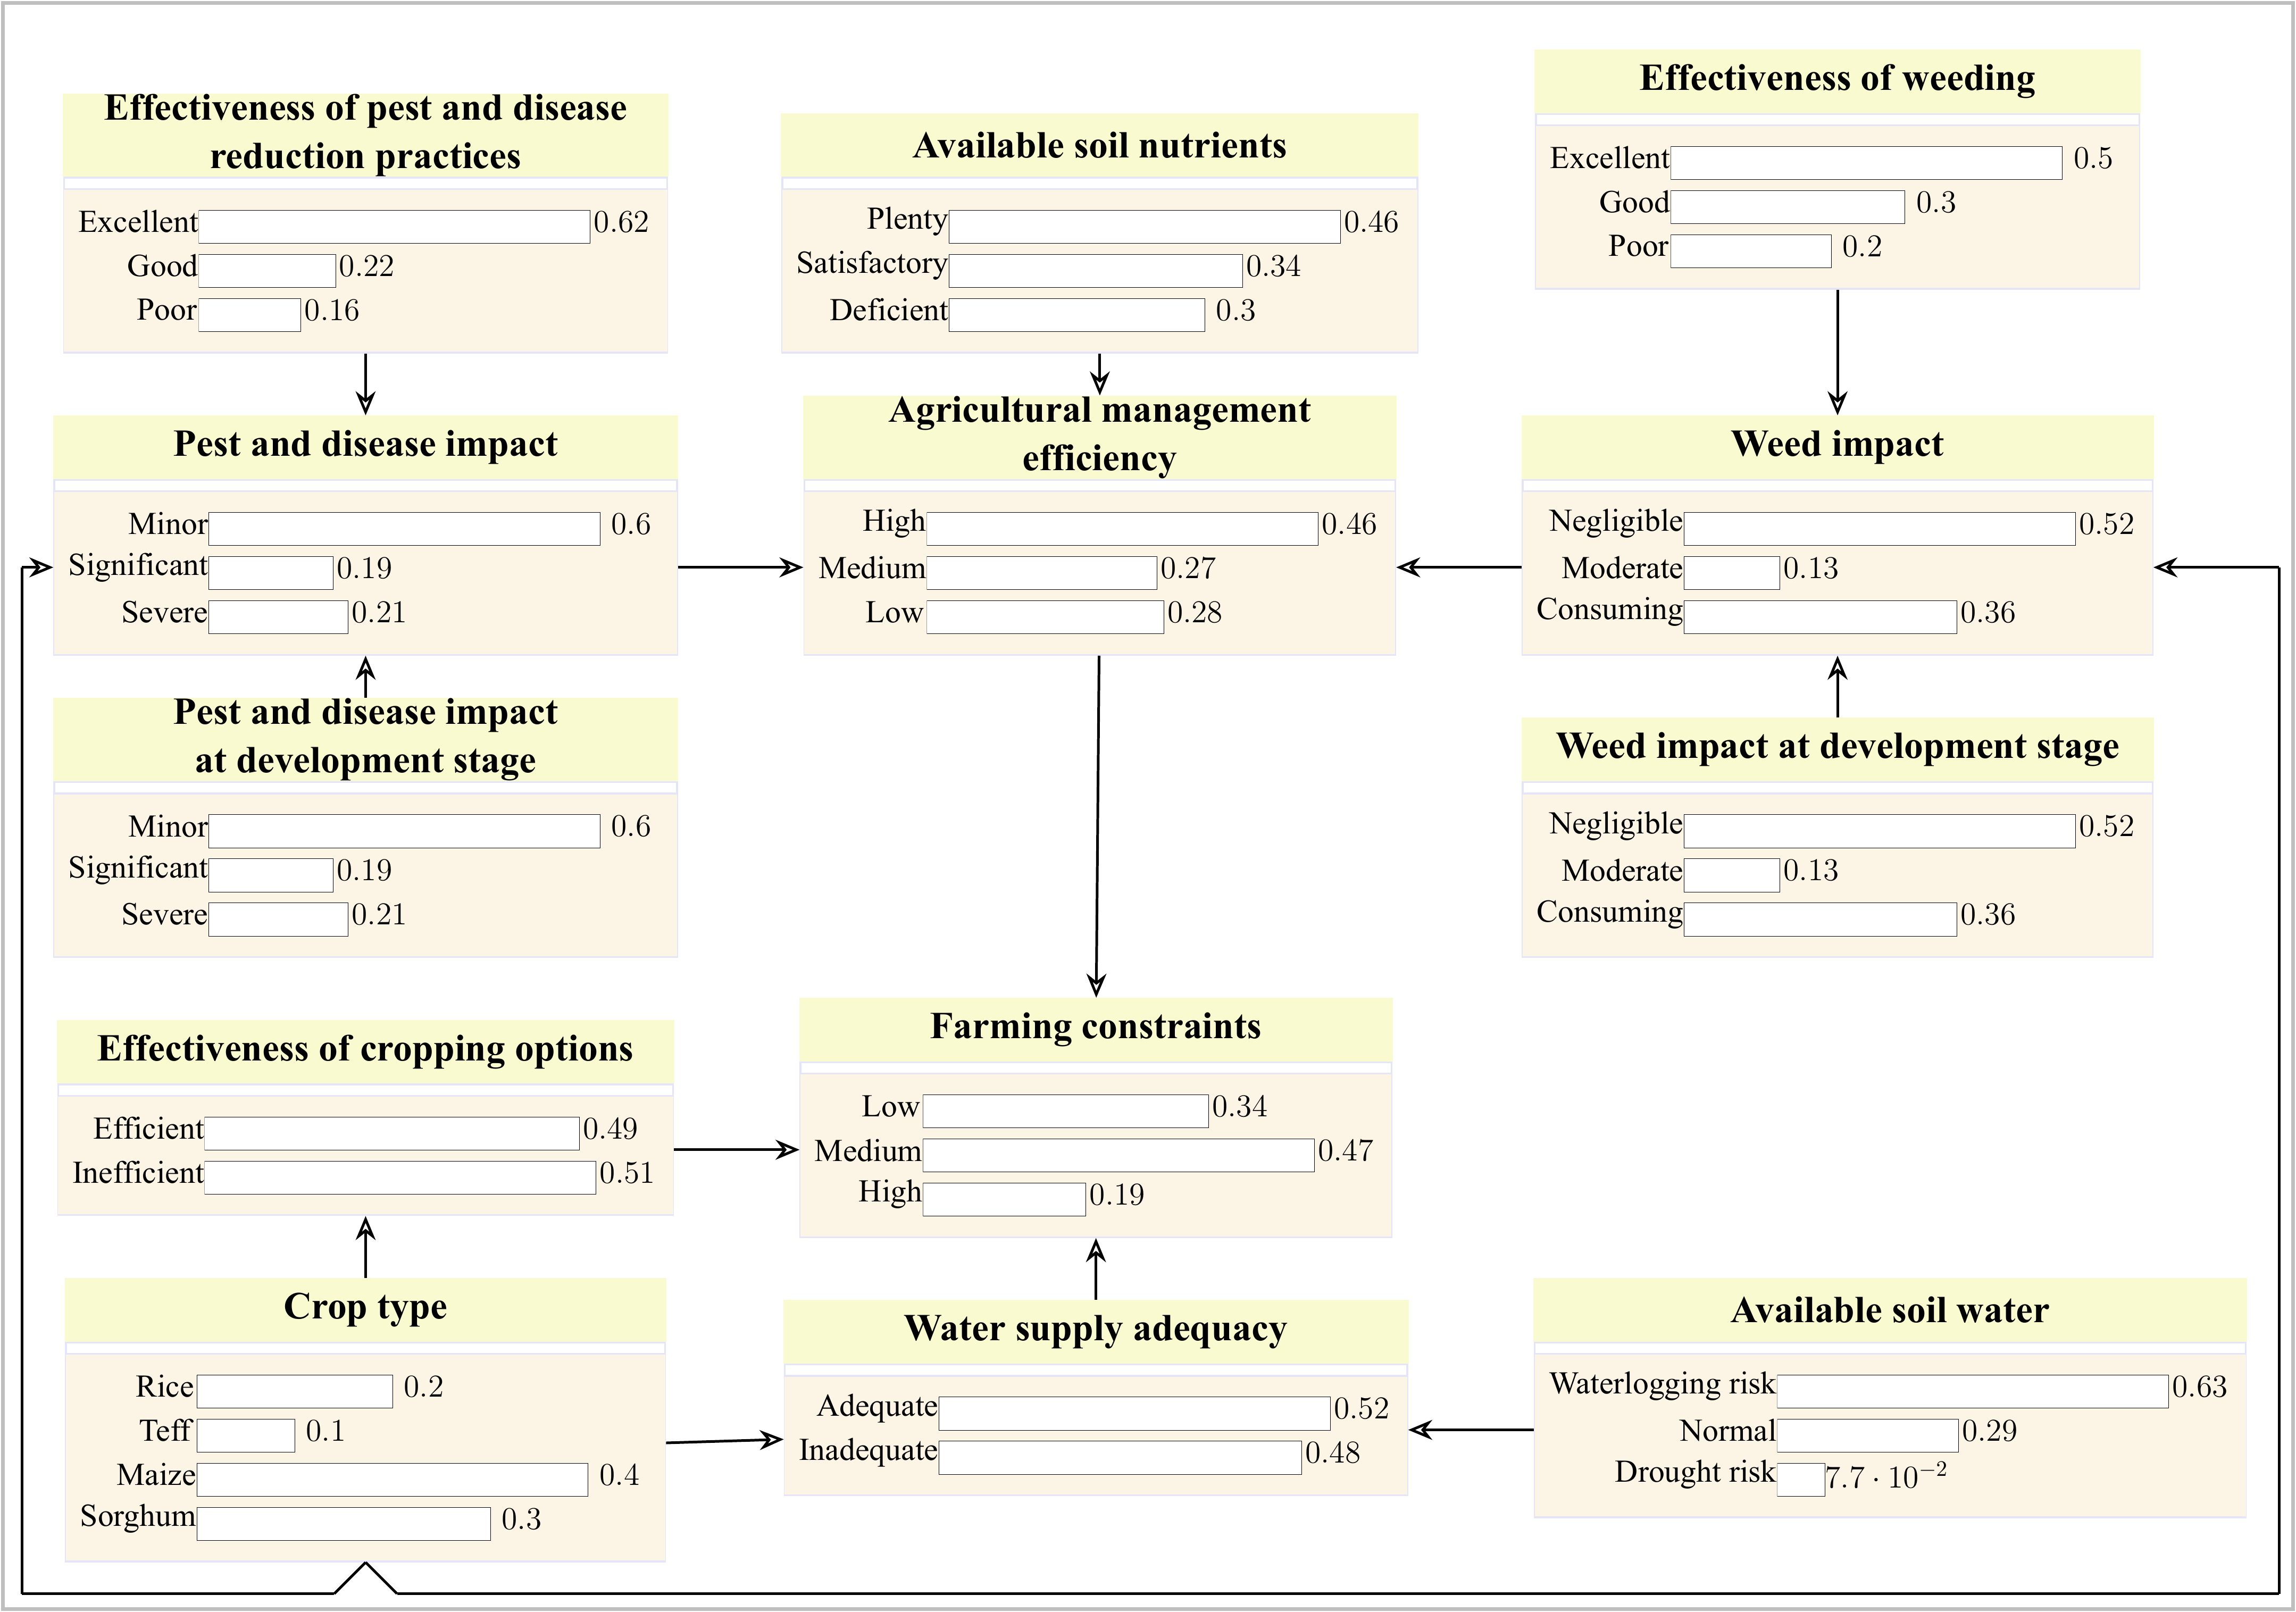
\includegraphics[width=1\linewidth,]{Modelling_FBFS_files/figure-latex/fig9-plot-1} 

}

\caption{Overview of causal relationships defining the farming constraints in flood-based farming systems in the Tigray region of Ethiopia and Kisumu County in Kenya.}\label{fig:fig9}
\end{figure}

The impacts of soil water and biotic stresses on grain yield suggest that crops subjected to strong farming constraints during early growth are likely to experience slow growth over the entire season. This cumulative effect of farming constraints seems to cause important biomass losses, which translate into low yields. Grain yield is very low when the late stage constraints are high, regardless of the states of pests \& diseases or water at the previous stages. Under such conditions, grain yield in both crops rarely exceeds 1 ton/ha. Grain yield expectations are generally higher in sorghum and more sensitive to varying levels of farming constraints. These findings highlight the importance of the early and late stage regarding grain yield in FBFS of the study areas and suggest a need for adequate management and crop protection during these critical stages of crop development. Even with good conditions at these stages, grain yields rarely reach 5 tons/ha for rice and sorghum.

\begin{figure}[!h]

{\centering 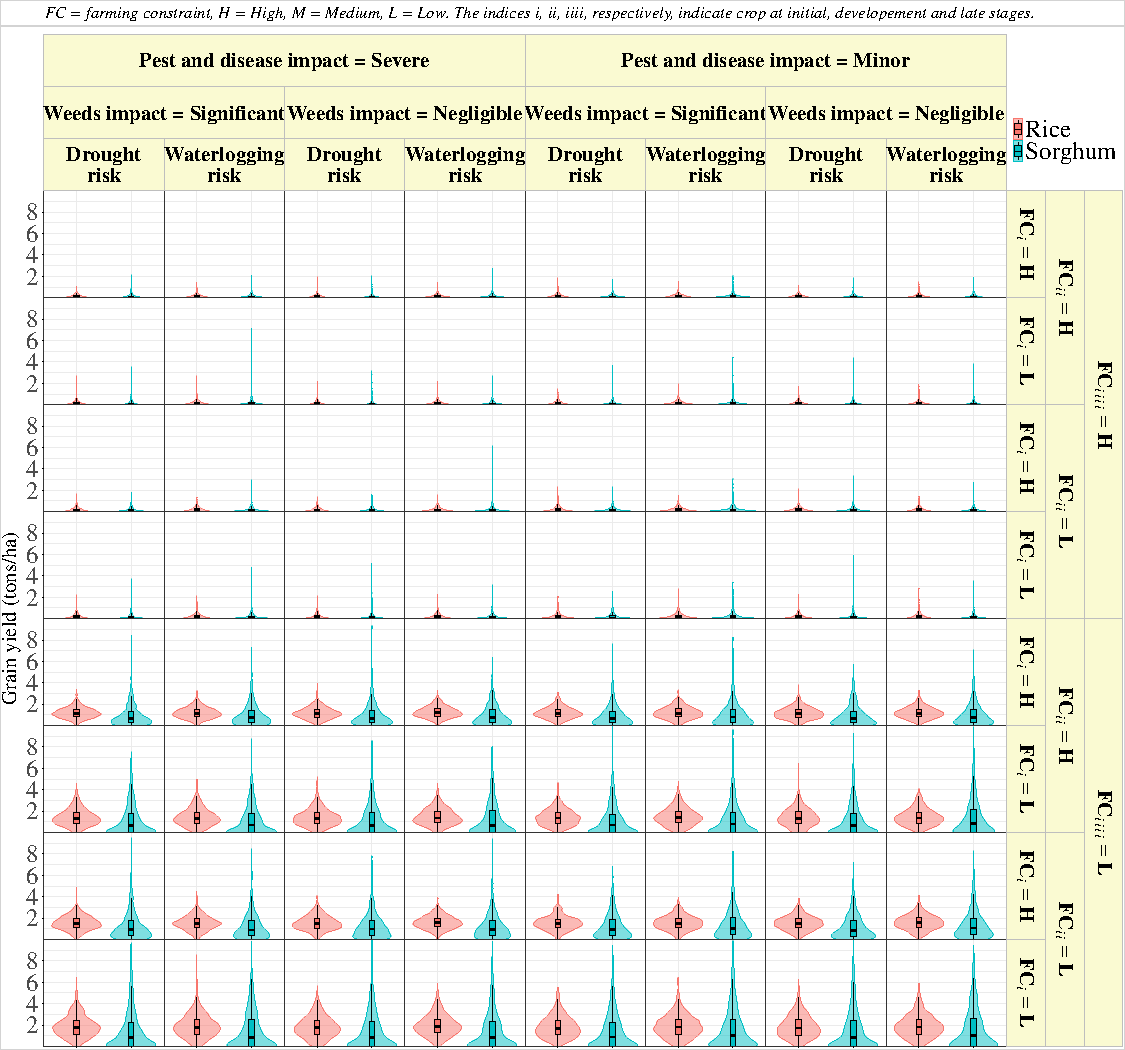
\includegraphics[width=1\linewidth,]{figures/Modelling_FBFS_grain_yield_violin_LOW} 

}

\caption{Effect of pests and diseases, weeds, and soil water on grain yield of rice and sorghum grown in flood-based farming systems in the Tigray region of Ethiopia and Kisumu County in Kenya. FC = farming constraint, H = High, M = Medium, L = Low. The indices i, ii, iiii, respectively, indicate crop at initial, development and late stages. Scenario for water, weed, pest and disease are taken at the mid stage of crop development. }\label{fig:fig10}
\end{figure}

Rice subjected to a high level of farming constraints during the initial and development stages seems insensitive to both water variation and changes in weed pressure. This may suggest that certain growth traits are affected by other forms of farming constraints than water and weeds, supporting the hypothesis of farming constraints during earlier growth being a major limitation to crop yield. However, controlling the level of pests \& diseases, supported by good water supply, is likely to be conducive to better yield regardless of weed levels. This suggests that efforts to control pests and diseases would be more effective than weed removal, when conditions are harsh during the earlier stages of rice development. Under limited water conditions and increasing levels of pests \& diseases, however, weed removal seems effective for improving grain yield in rice. This slight yield improvement seems to level off with better farm conditions at the development stage. These findings suggest possible rice-weed competition for water, which becomes irrelevant with better farm conditions. While weed removal generally improves rice grain yield, weeds are likely to have less of an effect when water is available, and pests and diseases are controlled. The effects of both weeds and pests \& diseases seem to increase with increasing soil moisture.

In contrast to rice, sorghum grown under high farming constraints at the initial and development stages seems to respond to varying levels of water and weeds. While the crop is likely to have higher yields with non-limiting water supply, it seems more suitable for drier conditions when severe pest \& disease effects are expected. However, in a situation of non-limited water supply, weed reduction only improves sorghum grain yield when the crop is exposed to strong pest \& disease impact. These results suggest that healthy sorghum is likely to be tolerant to a certain level of weeds, but weed removal may improve water productivity, particularly when weed-sorghum competition for space is limited. Regardless of water conditions, improved farm management at the early stage seems to improve the effect of weed removal in sorghum, particularly when the level of pest \& disease impact is minimal. With increased severity of pests \& diseases, sorghum seems to no longer respond to weed reduction. This implies the possibility of some sort of synergistic effect between these biotic stresses. When farm conditions are better at the development stage, both non-limiting water supply and weed reduction improve the yield of sorghum. This suggests that sorghum is more likely than other crops to escape from the farming constraint trap with improved management at later stages. When farm conditions are better at both initial and development stages, wetter conditions seem better under minimal pest \& disease pressure, whereas drier conditions are better in situations of severe pest and disease pressure. This supports the notion that moisture exacerbates the effect of pests \& diseases. In situations of limited pest \& disease impact, sorghum seems to respond to weed reduction only when water is limited. Under severe pest \& disease pressure, however, the crop seems to improve with weed removal regardless of the water conditions. This supports the findings on the cumulative effect of farming constraints and suggests possible weed-sorghum competition for water.

\hypertarget{ref5}{%
\section{Discussion}\label{ref5}}

The models presented in this paper navigate system complexity by breaking down a complex agricultural system into meaningful components, describing these components and bringing them together to provide a reasonable representation of the system. The participation of stakeholders and the inclusion of other relevant sources of information indicates that the model captured the necessary knowledge and can be used to support management decision in FBFS (Krueger et al., 2012; Refsgaard et al., 2007). This is important for crop models aiming to support agricultural development interventions, which requires realistic models. Because such models are often used as guidance for decision making, they must include hard-to-measure aspects, which often require non-trivial measurement and analysis methods. In doing so, a crop model for FBFS cannot ignore the various social aspects, which are crucial for crop production. While such aspects can be easily overlooked during model development or impossible to include without an adequate approach, crop models for agricultural decision support need to consider the whole system and represent at least its most important factors. This requires the inclusion of knowledge from different disciplines which, in turn, requires participatory approaches. In general, the traditional scientific method consisting of formulating and testing hypotheses is not suitable in this context due to at least 3 main reasons:

\begin{enumerate}
\def\labelenumi{\arabic{enumi}.}
\item
  \textbf{System simplification:} To study a specific aspect, traditional scientific methods must simplify the systems via the use of some sort of sampling method where functions and processes can be easily tested. While this approach has the merit of providing detail and generating knowledge, it is limited in producing a sufficiently comprehensive representation of the system of interest.
\item
  \textbf{The need for studying isolated aspects:} Isolated processes and functions must be connected to provide a holistic system representation, in which case further uncertainty due to interactions between these aspects must not be omitted.
\item
  \textbf{Resource constraints:} Time and resources are almost always limited, restricting the options to study individual aspects of the systems in detail.
\end{enumerate}

In attempting to guide decisions, crop models must recognize these aspects to make realistic recommendations based on the available information and resources. This means that such models must be framed in a way that allows the use of imperfect knowledge by the model. New knowledge and high-quality data constitute a means of reducing initial uncertainties, but they should not be a prerequisite to running a model in the first place.

These points should neither imply that hard data are not necessary, nor obscure the importance of detailed studies on individual system functions and processes, but highlight the need for recognizing the unknowns and acknowledging the intrinsic uncertainties in estimating them. The present study arises in a context where hard data are mostly unavailable, whereas practitioners and a small community of advisers and researchers are knowledgeable about the system of interest. Knowledge on 11 key aspects was required to achieve a reasonable representation of the system that seemed sufficient for making reliable predictions of crop performance and production risks. While few of the hundreds of variables included in the model were directly targeted by the study, each variable is crucial in defining system behaviour, hence should not be ignored when attempting to provide an artificial representation of the system. Removing a single variable may change the behaviour of the whole system and the overall prediction outcome, because the productivity of FBFS results from the interaction of many factors, such as soil fertility, water, and agricultural management.

Since the soil type is crucial for water supply (Figure \ref{fig:fig6}), soil properties can be important for the stability of water supply under specific settings. Clay soils can retain large amounts of water. Coarse sediments (i.e.~gravel or sand) have poor water holding capacity but benefit from finer components (i.e.~silt and clay). Because coarse sediments tend to be deposited first, upstream soils are more likely to have low water retention than downstream soils.

A major concern for FBFS farmers is the uncertainty surrounding the magnitude and intensity of flooding (Van Den Ham, 2008; Van Steenbergen et al., 2010). Water supply in FBFS is not determined by soil type or rainfall alone but also by availability and management of agronomic flooding and soil fertility, along with the social organisation involved at various scales. Harmful consequences of water supply (e.g.~drought, waterlogging) in a particular year can only be attenuated through adequate management. On soils with low water holding capacity (e.g.~sandy soils), the use of groundwater, which is relatively shallow due to the recurrent floods, can be considered for drought management. Groundwater from shallow wells can also constitute an additional source of drinking water. While soil fertility management can improve soil water conditions, the erosive effect of floodwater should not be underestimated. Rich soils are often transported between farmers' fields in the flood distribution network. The high risk of waterlogging on clayey and loamy soils can be addressed through limited tillage and enhanced soil organic matter content (Van Steenbergen et al., 2010).

The biomass produced in FBFS could be used to improve soil organic matter (Van Steenbergen et al., 2010), with two important challenges: restricted availability of crop residues due their use as fuel, and the lack of optimal interaction between crop and livestock. In many areas, crop residues are used as fuelwood for cooking with little returns of organic matter to the soil. This often results in reduced soil fertility, particularly in areas with limited fertilizer use. Livestock droppings constitute an important source of organic matter for FBFS, which serve as convenient post-harvest grazing areas. Where livestock pressure during such periods is high, treading can cause soil compaction. A possible management option could be the adoption of zero-grazing practices, where livestock are kept off-site and fed with crop residues, with manure subsequently transported back to the fields. This could be supplemented with composting to facilitate the decomposition of organic matter. Such innovations can have various effects on primary production at any crop development stage. Despite the high potential for biomass production, the net grain yield is strongly determined by farming constraints at the late stage of crop development (mainly pests and diseases; Figure \ref{fig:fig10}), which are crucial in the FBFS of the study areas. The cumulative effect and variability of farming constraints across farmlands (Figure \ref{fig:fig6}; Figure \ref{fig:fig8}; Figure \ref{fig:fig10}) stresses the importance of recognizing the complex web of processes that needs further investigation. Future research hypotheses can be centred on the nexus between four important aspects:

\begin{enumerate}
\def\labelenumi{\arabic{enumi}.}
\item
  Synergetic effects of different biotic stresses.
\item
  Sensitivity of different crops to the joint effect of these stresses.
\item
  Effect of water supply on different crops subjected to these stresses.
\item
  Options for managing these stresses for particular crops.
\end{enumerate}

When such aspects are well understood, experiments can be conducted to assess the attainable yield under reduced farming constraints and set realistic targets for closing the yield gap. According to Meng et al. (2013), three important factors are generally responsible for yield gaps. The first factor is a mismatch between the local climatic conditions and the crop cultivar, which does not allow exploitation of the entire available growing period. Inadequate sowing dates and thus relatively short-duration crops, can lead to earlier harvests than would be ideal, often not leaving enough time for crops to complete grain filling. In China, 7-15\% of yield losses have been attributed to harvest before physiological maturity (Meng et al., 2013). Yield losses in FBFS are exacerbated by harvest and post-harvest losses due to a range of pests and diseases (Figure \ref{fig:fig10}). In Kisumu for instance, rice farmers experience important losses due to bird attacks beside other limitations of high agricultural importance. Other less perceptible losses, such as those incurred due to harvesting technologies, or market opportunity losses due to the lack of storage facilities, contribute to low returns on agricultural investments (Van den Berg and Singels, 2013). The second factor is related to the inadequacy of input allocation (e.g.~inadequate water and nutrient supply). In Tigray, and to some extent also in Kisumu, few farmers are using recommended amounts of fertilizers, and many schemes are exposed to water shortage. The third major reason for yield shortfalls is poor management resulting in inadequate crop protection.

\hypertarget{conclusion-and-policy-recommendations}{%
\section{Conclusion and policy recommendations}\label{conclusion-and-policy-recommendations}}

This paper presents a mixed modelling approach for forecasting yields in complex farming systems. Using the example of Flood-Based Farming Systems we build a model using simple building blocks and imperfect information. We demonstrate how simple probabilistic tools can be combined to make predictions based on different scenarios that account for variability across farmlands within a farming system. We show how intangible factors can be assessed for inclusion into the model and how such seemingly less important factors can have cumulative effects on model predictions. We argue that crop models aiming to support development interventions should not underestimate the complexity of the farming systems and find ways to account for all factors deemed important for the functioning of the whole farming system. The study highlights the importance of systems analysis and offers suggestions for integrating different types of data and modelling approaches into farming system models.

The findings suggest that addressing farming constraints to reduce yield gaps can double the current crop production in FBFS of the study areas. These constraints include aspects such as uncertainty in water supply, or the production risk due to biotic stresses.

Risk management related to uncertainty in floodwater availability is perhaps the most important concern in FBFS settings. While most studies are currently focusing on the water delivery at various topographic scales, development interventions should concentrate on optimizing the little available floodwater via the use of adequate soil and water conservation techniques. These techniques should consider the soil type, the floodwater delivery and its uncertainty in space and time (e.g.~water source, water distribution networks, water acquisition structures), and more importantly, adequate management practices (e.g.~improving soil organic matter) for keeping the desired amount of this water within the root zone. This highlights the importance of pre-season management.

The importance of floodwater often masks that of other aspects that can be as important as water supply. While we found little hard data on the biotic stresses in FBFS settings, we found that these stressors can severely affect biomass accumulation and jeopardize grain yield. The prevailing moisture conditions of FBFS aggravate the impacts of these biotic stresses, and synergistic effects between these stressors cause further damage. Crop protection in FBFS should be a continuous effort, with early control promising the greatest success.

In general, the effect of farming constraints accumulates over time to the extent that crops can get trapped in a situation of slow growth affecting biomass accumulation and ultimately grain yield. We suspect the existence of a certain threshold beyond which biomass accumulation is slowed down, and another threshold beyond which crop growth becomes negligible. Net grain yield was found to depend strongly on late-stage constraints, which are mostly related to biotic stresses.

In a nutshell, development policies should focus on sustainable water supply and crop protection. Research and development should concentrate on closing the current FBFS yield gap through the study of farming constraints that compromise primary production. More studies, preferably in the form of quantitative estimates, are needed on biotic stresses and the factors that aggravate their impact on crop production.

\hypertarget{acknowledgements}{%
\section*{Acknowledgements}\label{acknowledgements}}
\addcontentsline{toc}{section}{Acknowledgements}

This study was funded by the Deutscher Akademischer Austauschdienst (DAAD) and the World Agroforestry Centre (ICRAF). We thank the farmers and experts who contributed in various ways during the development of the model. We thank the department of Dryland Agriculture of Mekelle University for guidance on the sampling frame in the Tigray region and for facilitating logistics during field work. Thanks to the participants of the leadership course in flood-based farming and water harvesting in Kenya and the participants of the International Training on Integrated Watershed Management and FBFS in Ethiopia, who drafted the models.

\hypertarget{references}{%
\section*{References}\label{references}}
\addcontentsline{toc}{section}{References}

\hypertarget{refs}{}
\leavevmode\hypertarget{ref-Allen_et_al_1998}{}%
Allen, R.G., Pereira, L.S., Raes, D., Smith, M., 1998. Crop evapotranspiration: Guidelines for computing crop requirements, FAO irrigation and drainage papers (book 56). FAO, Rome.

\leavevmode\hypertarget{ref-Baroni_and_Tarantola_2014}{}%
Baroni, G., Tarantola, S., 2014. A General Probabilistic Framework for uncertainty and global sensitivity analysis of deterministic models: A hydrological case study. Environmental Modelling \& Software 51, 26--34. \url{https://doi.org/10.1016/j.envsoft.2013.09.022}

\leavevmode\hypertarget{ref-Belgorodski_et_al_2017}{}%
Belgorodski, N., Greiner, M., Tolksdorf, K., Schueller, K., 2017. rriskDistributions: Fitting distributions to given data or known quantiles. The Comprehensive R Archive Network.

\leavevmode\hypertarget{ref-Boote_et_al_1996}{}%
Boote, K.J., Jones, J.W., Pickering, N.B., 1996. Potential Uses and Limitations of Crop Models. Agronomy Journal 88, 704--716. \url{https://doi.org/10.2134/agronj1996.00021962008800050005x}

\leavevmode\hypertarget{ref-Delignette-Muller_and_Dutang_2015}{}%
Delignette-Muller, M.L., Dutang, C., 2015. fitdistrplus : An R Package for Fitting Distributions. Journal of Statistical Software 64, 1--34. \url{https://doi.org/10.18637/jss.v064.i04}

\leavevmode\hypertarget{ref-Erkossa_et_al_2014}{}%
Erkossa, T., Langan, S.J., Hagos, F., 2014. Constraints to the development, operation and maintenance of spate irrigation schemes in Ethiopia., in: Erkossa, Teklu; Hagos, Fitsum; Lefore, N. (Ed.), Proceedings of the Workshop on Flood-Based Farming for Food Security and Adaption to Climate Change in Ethiopia: Potential and Challenges. International Water Management Institute (IWMI), Adama, pp. 5--22. \url{https://doi.org/https://dx.doi.org/10.5337/2014.233}

\leavevmode\hypertarget{ref-FBLN_2018}{}%
FBLN, 2018. Flood-based Livelihood Network (FBLN) Foundation.

\leavevmode\hypertarget{ref-Fenton_and_Neil_2013}{}%
Fenton, N., Neil, M., 2013. Risk Assessment and Decision Analysis With Bayesian Networks. CRC Press, Boca Raton.

\leavevmode\hypertarget{ref-Gallagher_1987}{}%
Gallagher, P., 1987. U.S. Soybean Yields: Estimation and Forecasting with Nonsymmetric Disturbances. American Journal of Agricultural Economics 69, 796--803. \url{https://doi.org/10.2307/1242190}

\leavevmode\hypertarget{ref-Haile_2010}{}%
Haile, A.M., 2010. A Tradition in Transition, Water Management Reforms and Indigenous Spate Irrigation Systems in Eritrea, 1st ed. CRC Press, London.

\leavevmode\hypertarget{ref-Hansson_and_Sjokvist_2013}{}%
Hansson, F., Sjökvist, S., 2003. Modelling Expert Judgement into a Bayesian Belief Network - A Method for Consistent and Robust Determination of Conditional Probability Tables (Master's thesis). Mathematical Statistics, LUND University.

\leavevmode\hypertarget{ref-Harlan_and_Pasquereau_1969}{}%
Harlan, J.R., Pasquereau, J., 1969. Décrue Agriculture in Mali. Economic Botany 23, 70--74. \url{https://doi.org/10.1007/BF02862973}

\leavevmode\hypertarget{ref-Hubbard_2014}{}%
Hubbard, D.W., 2014. How to Measure Anything: Finding the Value of Intangibles in Business, 3rd ed. ed. John Wiley \& Sons, Inc., Hoboken.

\leavevmode\hypertarget{ref-Hojsgaard_2012}{}%
Højsgaard, S., 2012. Graphical Independence Networks with the gRain Package for R. Journal of Statistical Software 46, 1--26. \url{https://doi.org/10.18637/jss.v046.i10}

\leavevmode\hypertarget{ref-Jax_and_Setala_2005}{}%
Jax, K., Setälä, H., 2005. Function and "Functioning" in Ecology: What Does It Mean? Oikos 111, 641--648.

\leavevmode\hypertarget{ref-Jensen_1996}{}%
Jensen, F.V., 1996. An Introduction of Bayesian Network, 1st ed. Springer; Har/Dskt edition, Heidelberg.

\leavevmode\hypertarget{ref-Junk_et_al_1989}{}%
Junk, W., Bayley, P., Sparks, R., 1989. The Flood Pulse Concept in River - Floodplain Systems, in: Dodge, D.P. (Ed.), Proceedings of the International Large River Symposium. Can. Spec. Publ, Honey Harbour, pp. 110--127.

\leavevmode\hypertarget{ref-Kitagawa_1996}{}%
Kitagawa, G., 1996. Monte Carlo Filter and Smoother for Non-Gaussian Nonlinear State Space Models. Journal of Computational and Graphical Statistics 5, 1--25. \url{https://doi.org/10.2307/1390750}

\leavevmode\hypertarget{ref-Koller_and_Friedman_2009}{}%
Koller, D., Friedman, N., 2009. Probabilistic Graphical Models: Principles and Techniques, 1st ed. MIT Press, Cambridge.

\leavevmode\hypertarget{ref-Krueger_et_al_2012}{}%
Krueger, T., Page, T., Hubacek, K., Smith, L., Hiscock, K., 2012. The role of expert opinion in environmental modelling. Environmental Modelling and Software 36, 4--18. \url{https://doi.org/https://doi.org/10.1016/j.envsoft.2012.01.011}

\leavevmode\hypertarget{ref-Luedeling_Goehring_et_al_2019}{}%
Luedeling, E., Goehring, L., Schiffers, K., 2019. decisionSupport: Quantitative support of decision making under uncertainty. The Comprehensive R Archive Network.

\leavevmode\hypertarget{ref-Luedeling_et_al_2015}{}%
Luedeling, E., Oord, A.L., Kiteme, B., Ogalleh, S., Malesu, M., Shepherd, K.D., De Leeuw, J., 2015. Fresh groundwater for Wajir - ex-ante assessment of uncertain benefits for multiple stakeholders in a water supply project in Northern Kenya. Frontiers in Environmental Science 3. \url{https://doi.org/10.3389/fenvs.2015.00016}

\leavevmode\hypertarget{ref-Luedeling_and_Shepherd_2016}{}%
Luedeling, E., Shepherd, K., 2016. Decision-Focused Agricultural Research. Solutions 7, 46--54.

\leavevmode\hypertarget{ref-Meng_et_al_2013}{}%
Meng, Q., Hou, P., Wu, L., Chen, X., Cui, Z., Zhang, F., 2013. Understanding production potentials and yield gaps in intensive maize production in China. Field Crops Research 143, 91--97. \url{https://doi.org/10.1016/j.fcr.2012.09.023}

\leavevmode\hypertarget{ref-Murthy_2004}{}%
Murthy, V.R.K., 2004. Crop Growth Modeling and Its Applications in Agricultural Meteorology, in: Sivakumar, M.V., Roy, P.S., Harmsen, K., Saha, S.K. (Eds.), Satellite Remote Sensing and Gis Applications in Agricultural Meteorology. World Meteorological Organisation, Dehra Dun, pp. 235--261.

\leavevmode\hypertarget{ref-Pearl_1988}{}%
Pearl, J., 1988. Probabilistic Reasoning in Intelligent Systems: Networks of Plausible Inference. Morgan Kaufmann Publishers Inc., San Francisco.

\leavevmode\hypertarget{ref-Ramirez_et_al_2003}{}%
Ramirez, O.A., Misra, S., Field, J., 2003. Crop‐Yield Distributions Revisited. American Journal of Agricultural Economics 85, 108--120. \url{https://doi.org/10.1111/1467-8276.00106}

\leavevmode\hypertarget{ref-R_Core_Team_2019}{}%
R Core Team, 2019. R: A language and environment for statistical computing. R Foundation for Statistical Computing, Vienna, Austria.

\leavevmode\hypertarget{ref-Refsgaard_et_al_2007}{}%
Refsgaard, J.C., Sluijs, J.P. van der, Højberg, A.L., Vanrolleghem, P.A., 2007. Uncertainty in the environmental modelling process - A framework and guidance. Environmental Modelling and Software 22, 1543--1556. \url{https://doi.org/https://doi.org/10.1016/j.envsoft.2007.02.004}

\leavevmode\hypertarget{ref-Rosenstock_et_al_2014}{}%
Rosenstock, T.S., Mpanda, M., Rioux, J., Aynekulu, E., Kimaro, A.A., Neufeldt, H., Shepherd, K.D., Luedeling, E., 2014. Targeting conservation agriculture in the context of livelihoods and landscapes. Agriculture, Ecosystems and Environment 187, 47--51. \url{https://doi.org/10.1016/j.agee.2013.11.011}

\leavevmode\hypertarget{ref-Scutari_2010}{}%
Scutari, M., 2010. Learning Bayesian Networks with the bnlearn R Package. Journal of Statistical Software 35, 1--22. \url{https://doi.org/10.18637/jss.v035.i03}

\leavevmode\hypertarget{ref-Scutari_and_Denis_2015}{}%
Scutari, M., Denis, J.-B., 2015. Networks Bayesian With Examples in R, 1st ed. CRC Press, Boca Raton.

\leavevmode\hypertarget{ref-Uusitalo_et_al_2015}{}%
Uusitalo, L., Lehikoinen, A., Helle, I., Myrberg, K., 2015. An overview of methods to evaluate uncertainty of deterministic models in decision support. Environmental Modelling and Software 63, 24--31. \url{https://doi.org/10.1016/j.envsoft.2014.09.017}

\leavevmode\hypertarget{ref-VandenBerg_and_Singels_2013}{}%
Van den Berg, M., Singels, A., 2013. Modelling and monitoring for strategic yield gap diagnosis in the South African sugar belt. Field Crops Research 143, 143--150. \url{https://doi.org/10.1016/j.fcr.2012.10.009}

\leavevmode\hypertarget{ref-Van_den_Ham_2008}{}%
Van Den Ham, J.-P., 2008. Dodota Spate Irrigation System Ethiopia - A case study of Spate Irrigation Management and Livelihood options (Master's thesis). Wageningen University.

\leavevmode\hypertarget{ref-VanIttersum_et_al_2013}{}%
Van Ittersum, M.K., Cassman, K.G., Grassini, P., Wolf, J., Tittonell, P., Hochman, Z., 2013. Yield gap analysis with local to global relevance-A review. Field Crops Research 143, 4--17. \url{https://doi.org/10.1016/j.fcr.2012.09.009}

\leavevmode\hypertarget{ref-VanSteenbergen_et_al_2011a}{}%
Van Steenbergen, F., Haile, A.M., Alemehayu, T., Alamirew, T., Geleta, Y., 2011. Status and Potential of Spate Irrigation in Ethiopia. Water Resources Management 25, 1899--1913. \url{https://doi.org/10.1007/s11269-011-9780-7}

\leavevmode\hypertarget{ref-VanSteenbergen_et_al_2010}{}%
Van Steenbergen, F., Lawrence, P., Haile, A.M., Salman, M., Faurès, J.-M., 2010. Guidelines on spate irrigation. FAO, Rome.

\leavevmode\hypertarget{ref-Whitney_Lanzanova_et_al_2018}{}%
Whitney, C., Lanzanova, D., Muchiri, C., Shepherd, K.D., Rosenstock, T.S., Krawinkel, M., Tabuti, J.R.S., Luedeling, E., 2018. Probabilistic Decision Tools for Determining Impacts of Agricultural Development Policy on Household Nutrition. Earth's Future 6, 359--372. \url{https://doi.org/10.1002/2017EF000765}

\leavevmode\hypertarget{ref-Whitney_Shepherd_et_al_2018}{}%
Whitney, C., Shepherd, K., Luedeling, E., 2018. Decision analysis methods guide; Agricultural policy for nutrition (No. 275). World Agroforestry Centre, Nairobi. \url{https://doi.org/10.5716/WP18001.PDF}

\leavevmode\hypertarget{ref-Yet_et_al_2016}{}%
Yet, B., Constantinou, A., Fenton, N., Neil, M., Luedeling, E., Shepherd, K., 2016. A Bayesian Network Framework for Project Cost, Benefit and Risk Analysis with an Agricultural Development Case Study. Expert Systems with Applications 60, 141--155. \url{https://doi.org/10.1016/j.eswa.2016.05.005}


\end{document}


